% !TEX program = pdflatex
% !TEX encoding = UTF-8 Unicode

\documentclass{beamer}
\usepackage[utf8]{inputenc}
\usepackage[T1]{fontenc}
\usepackage{lmodern}
\usepackage{amsmath,amssymb}
\usepackage{graphicx}
\usepackage{booktabs}
\usepackage{hyperref}

\usetheme{Madrid}
\usecolortheme{default}

% Custom colors for better visuals
\definecolor{darkblue}{RGB}{0,51,102}
\definecolor{lightblue}{RGB}{173,216,230}
\setbeamercolor{structure}{fg=darkblue}

%------------------------------------------------------------
% Title page configuration
%------------------------------------------------------------
\title[PCG Arena]{PCG Arena}
\subtitle{A Web Platform for Blind A/B Testing of\\Procedural Content Generators}

\author{Antoni Czapski}

\institute[]{
  Artificial Intelligence $\heartsuit$ Games:\\
  Procedural Content Generation
}

\date{February 2026}

% Graphics path
\graphicspath{{../latex/img/}}

%------------------------------------------------------------
% Table of contents at each section
%------------------------------------------------------------
\AtBeginSection[]
{
  \begin{frame}
    \frametitle{Outline}
    \tableofcontents[currentsection]
  \end{frame}
}

%------------------------------------------------------------
\begin{document}

%------------------------------------------------------------
% Title
%------------------------------------------------------------
\frame{\titlepage}

%------------------------------------------------------------
% Table of Contents
%------------------------------------------------------------
\begin{frame}
\frametitle{Outline}
\tableofcontents
\end{frame}

%==============================================================================
\section{Motivation \& Problem}
%==============================================================================

%------------------------------------------------------------
\begin{frame}
\frametitle{The PCG Evaluation Problem}

\begin{columns}
\column{0.55\textwidth}
\textbf{Challenge:} How do we know if a PCG algorithm produces ``good'' levels?

\vspace{0.5em}
\begin{itemize}
    \item Automated metrics miss \alert{player experience}
    \item Lab studies have \alert{limited participants}
    \item Generator reputation creates \alert{bias}
\end{itemize}

\vspace{0.5em}
\textbf{Solution:} Web-based blind A/B testing at scale

\column{0.45\textwidth}
\begin{block}{Research Questions}
\begin{enumerate}
    \item What makes levels ``good''?
    \item Are player preferences consistent?
    \item Can we build a reward model?
\end{enumerate}
\end{block}
\end{columns}

\end{frame}

%------------------------------------------------------------
\begin{frame}
\frametitle{PCG Arena: Core Concept}

\begin{center}
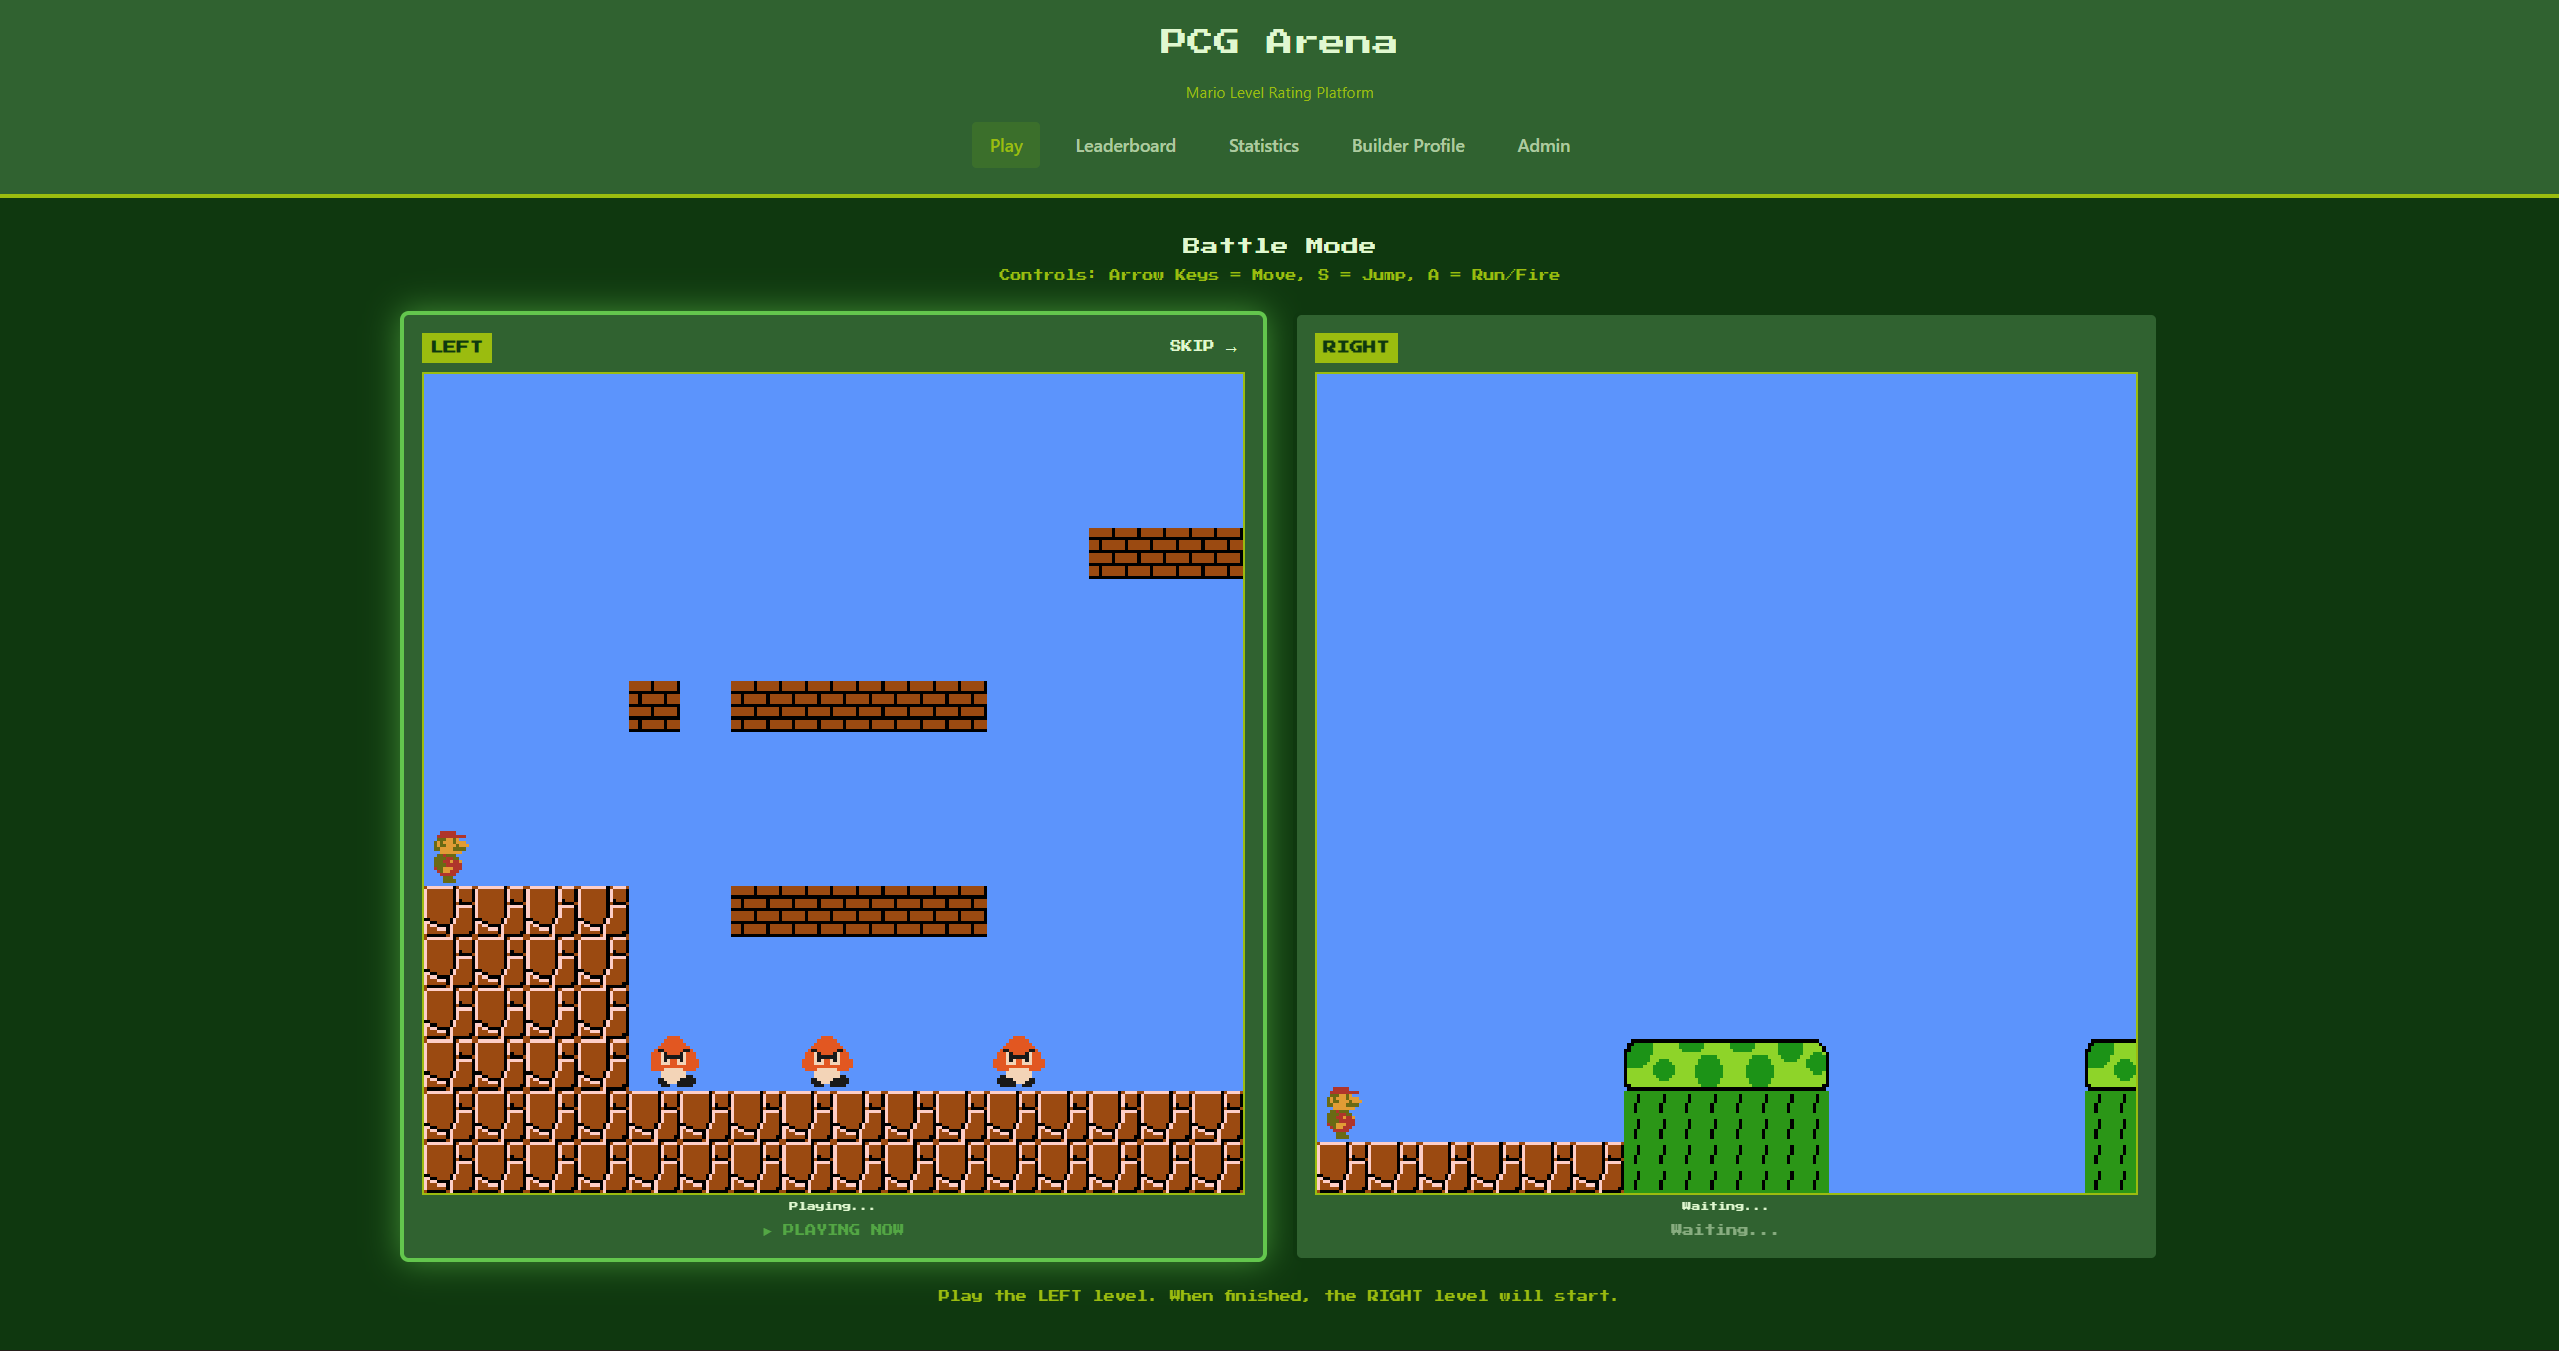
\includegraphics[width=0.85\textwidth]{main_gameplay.png}
\end{center}

\vspace{-0.5em}
\begin{itemize}
    \item Play two levels $\rightarrow$ Vote for favorite $\rightarrow$ Glicko-2 ranking
    \item \textbf{15 generators}, \textbf{748 levels}, \textbf{571 votes} collected
\end{itemize}

\end{frame}

%==============================================================================
\section{Platform Overview}
%==============================================================================

%------------------------------------------------------------
\begin{frame}
\frametitle{System Architecture}

\begin{columns}
\column{0.5\textwidth}
\textbf{Frontend}
\begin{itemize}
    \item React + TypeScript
    \item Mario engine ported from Java
    \item Browser-based gameplay
\end{itemize}

\vspace{0.5em}
\textbf{Backend}
\begin{itemize}
    \item FastAPI (Python)
    \item Glicko-2 rating system
    \item AGIS matchmaking
\end{itemize}

\column{0.5\textwidth}
\textbf{Infrastructure}
\begin{itemize}
    \item Docker containers
    \item Google Cloud Platform
    \item SQLite database
\end{itemize}

\vspace{0.5em}
\textbf{Live at:}
\begin{center}
\alert{\url{https://pcg-arena.com}}
\end{center}
\end{columns}

\end{frame}

%------------------------------------------------------------
\begin{frame}
\frametitle{Key Platform Features}

\begin{columns}
\column{0.5\textwidth}

\begin{block}{For Players}
\begin{itemize}
    \item No download required
    \item Google OAuth login
    \item Tag gameplay characteristics
\end{itemize}
\end{block}

\begin{block}{For Researchers}
\begin{itemize}
    \item Submit custom generators
    \item View live leaderboard
    \item Export research data
\end{itemize}
\end{block}

\column{0.5\textwidth}
\begin{center}
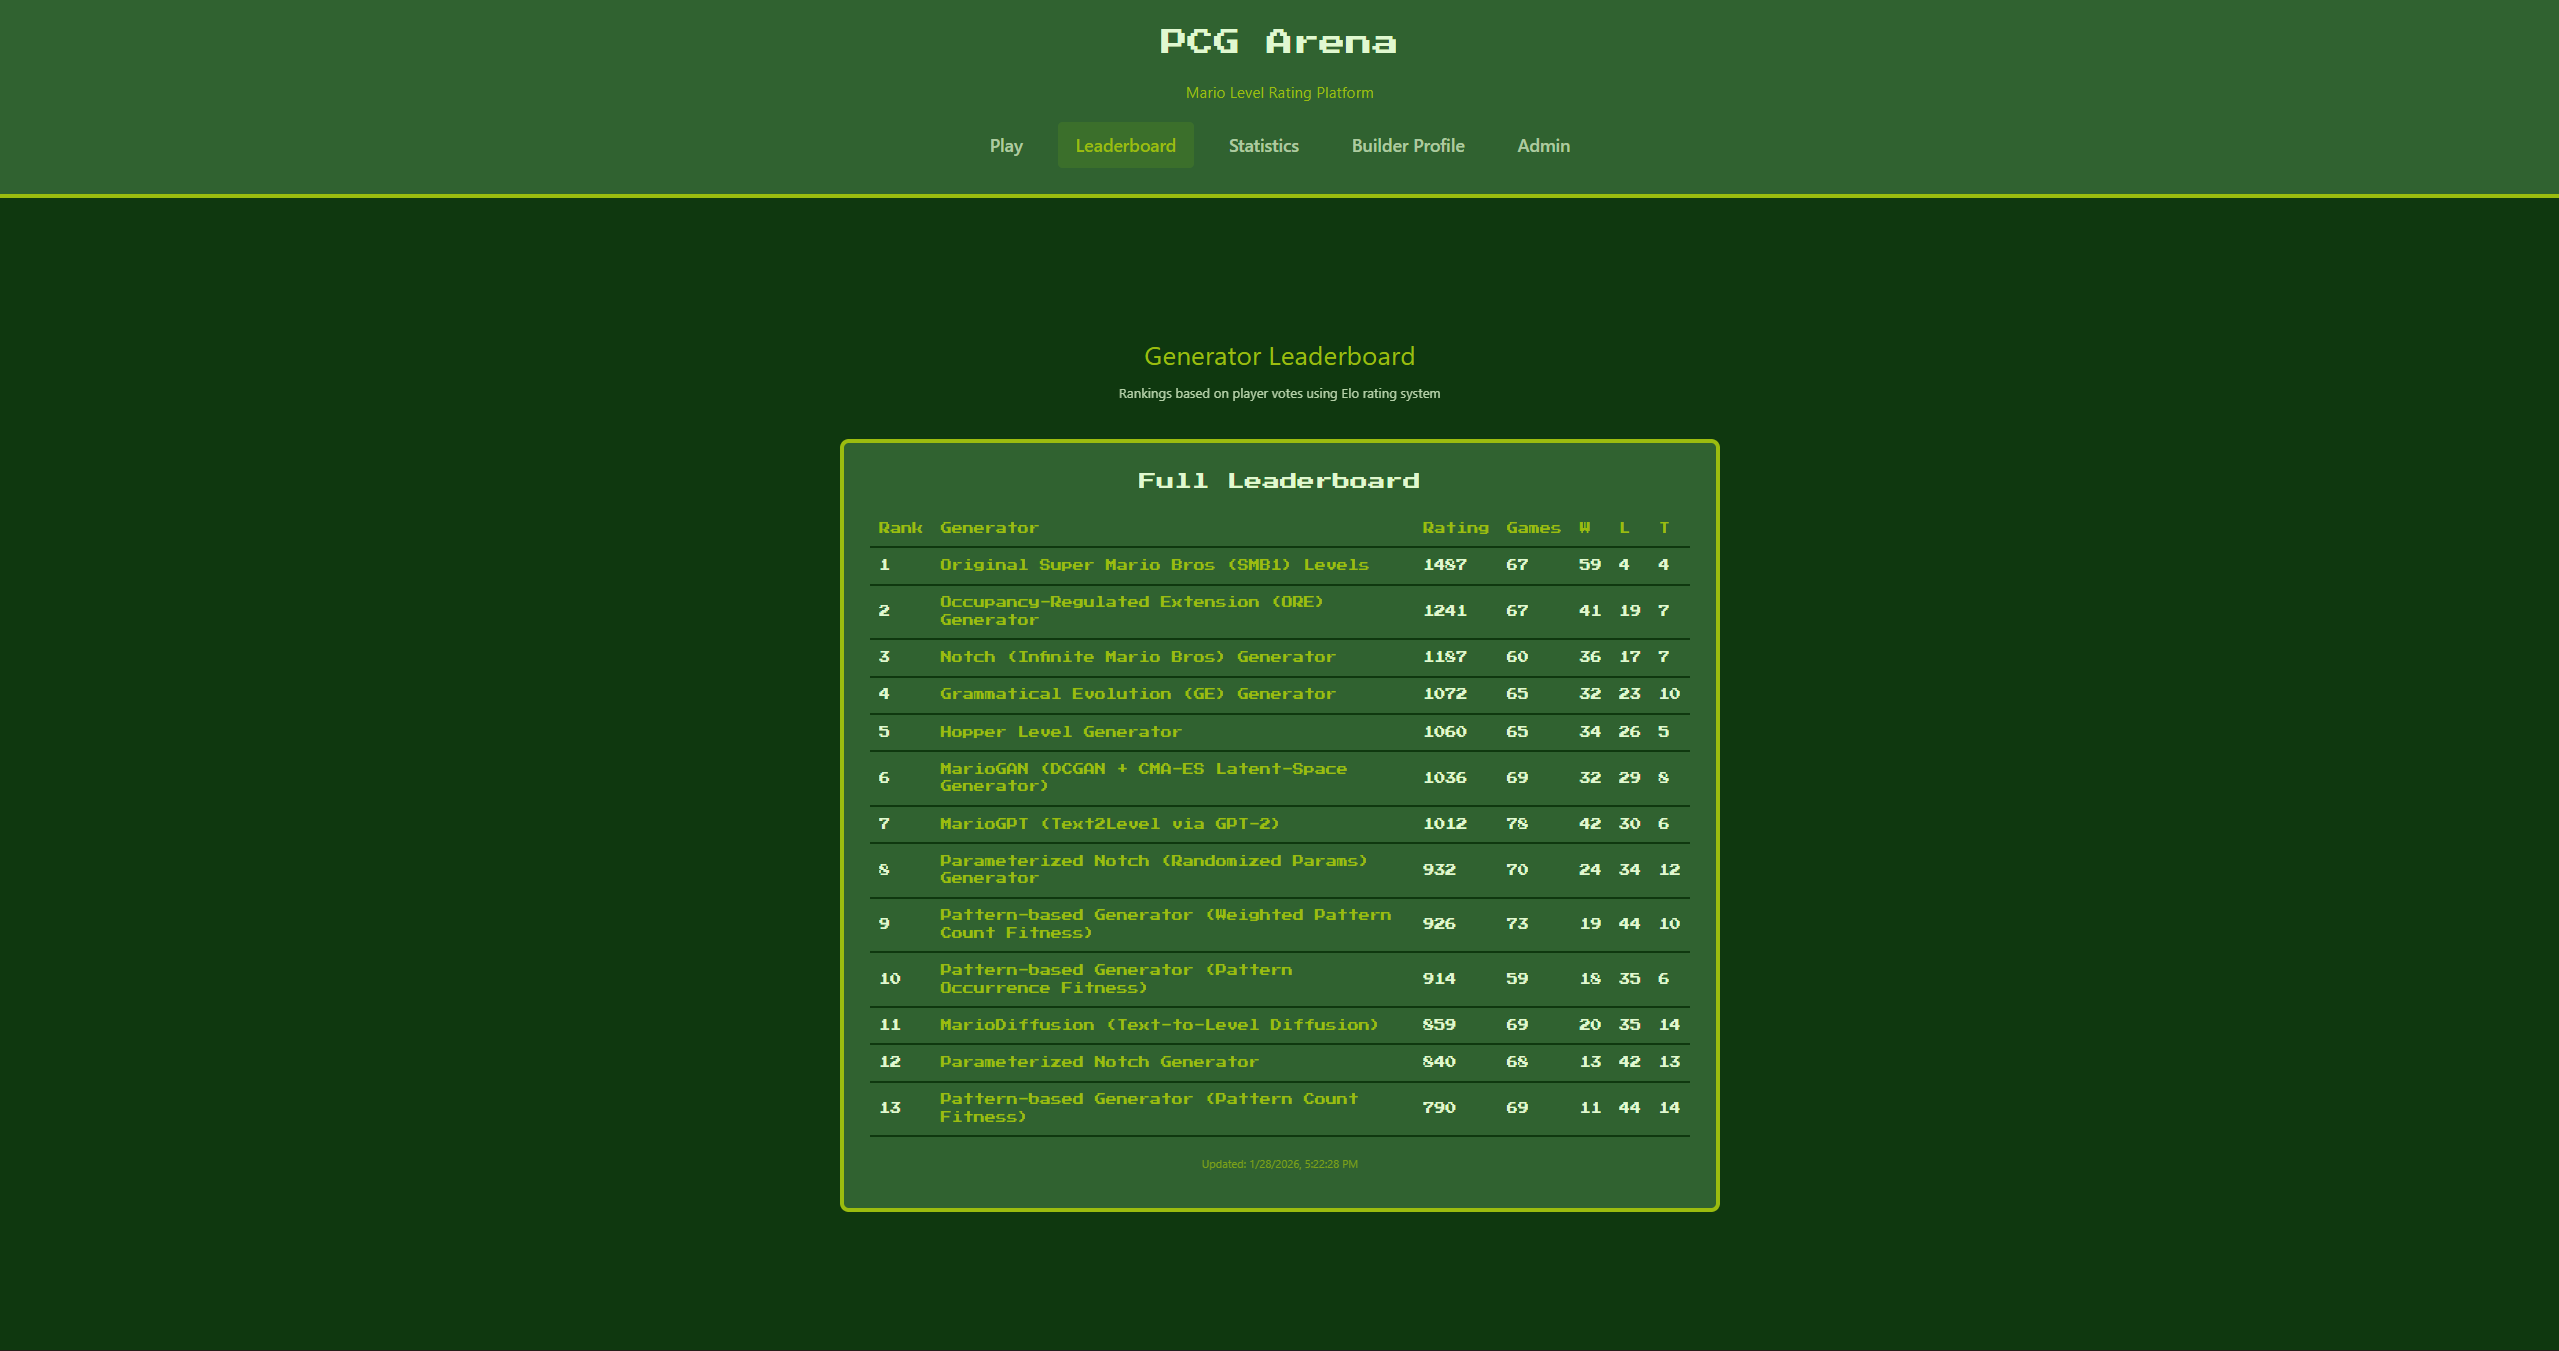
\includegraphics[width=\textwidth]{leaderboard.png}
\end{center}
\end{columns}

\end{frame}

%------------------------------------------------------------
\begin{frame}
\frametitle{Glicko-2 Rating System}

\begin{columns}
\column{0.55\textwidth}
\textbf{Why Glicko-2?}
\begin{itemize}
    \item Provides \alert{uncertainty estimates} (RD)
    \item Handles \alert{inactive} generators
    \item Maps pairwise comparisons to rankings
\end{itemize}

\vspace{0.5em}
\textbf{Win probability:}
$$P(A \text{ wins}) = \frac{1}{1 + 10^{(R_B - R_A)/400}}$$

\column{0.45\textwidth}
\begin{table}
\centering
\footnotesize
\begin{tabular}{lr}
\toprule
\textbf{Parameter} & \textbf{Value} \\
\midrule
Initial Rating & 1000 \\
Initial RD & 350 \\
System $\tau$ & 0.5 \\
\bottomrule
\end{tabular}
\caption{Glicko-2 settings}
\end{table}
\end{columns}

\end{frame}

%==============================================================================
\section{Generators Under Test}
%==============================================================================

%------------------------------------------------------------
\begin{frame}
\frametitle{14 PCG Algorithms Compared}

\begin{columns}
\column{0.5\textwidth}
\textbf{Neural/ML-Based}
\begin{itemize}
    \item MarioGPT (GPT-2)
    \item MarioGAN (DCGAN)
    \item MarioDiffusion
    \item MarioDPO \alert{(ours)}
\end{itemize}

\vspace{0.5em}
\textbf{Search-Based}
\begin{itemize}
    \item Genetic algorithm
    \item Hopper (agent simulation)
\end{itemize}

\column{0.5\textwidth}
\textbf{Grammar/Pattern-Based}
\begin{itemize}
    \item Notch variants (3)
    \item Pattern-based (3)
    \item ORE (occupancy)
\end{itemize}

\vspace{0.5em}
\textbf{Baseline}
\begin{itemize}
    \item \textbf{Original SMB} (15 levels)
\end{itemize}
\end{columns}

\vspace{0.5em}
\begin{center}
\alert{100 levels per generator} (except Original: 15)
\end{center}

\end{frame}

%==============================================================================
\section{Experiments \& Results}
%==============================================================================

%------------------------------------------------------------
\begin{frame}
\frametitle{RQ1: What Makes a Good Level?}

\begin{block}{H1: Flow Channel Hypothesis}
\textbf{Hypothesis:} Moderate difficulty (15--40\% death rate) maximizes enjoyment.\\
\textbf{Result:} \alert{Not Supported} -- Linear relationship: easier $=$ better ($r=-0.227$, $p=0.046$)
\end{block}

\begin{columns}
\column{0.5\textwidth}
\begin{center}
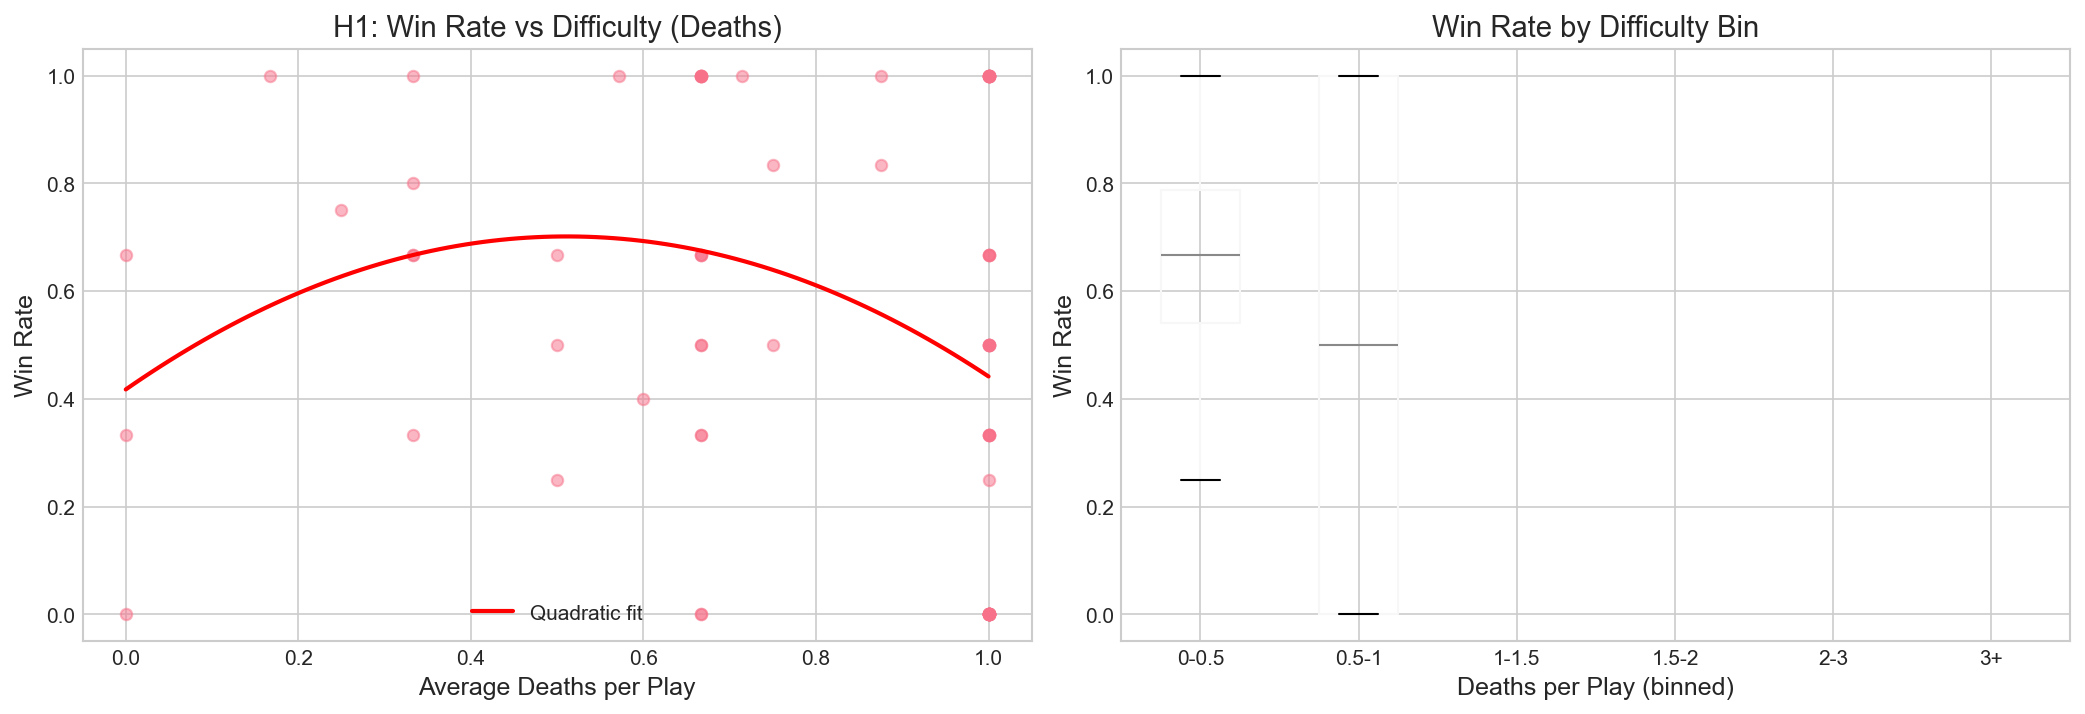
\includegraphics[width=\textwidth]{h1_difficulty_vs_winrate.png}
\end{center}

\column{0.5\textwidth}
\begin{block}{Conclusion}
Players prefer levels they can \alert{complete}. No inverted-U pattern found.
\end{block}
\end{columns}

\end{frame}

%------------------------------------------------------------
\begin{frame}
\frametitle{RQ1: Structural Variety}

\begin{block}{H2: Creativity Hypothesis}
\textbf{Hypothesis:} Higher terrain variety and enemy diversity preferred.\\
\textbf{Result:} \alert{Partially Supported} -- ``Creative'' tag $\leftrightarrow$ wins ($r=0.42$, $p<0.01$)
\end{block}

\begin{columns}
\column{0.5\textwidth}
\begin{center}
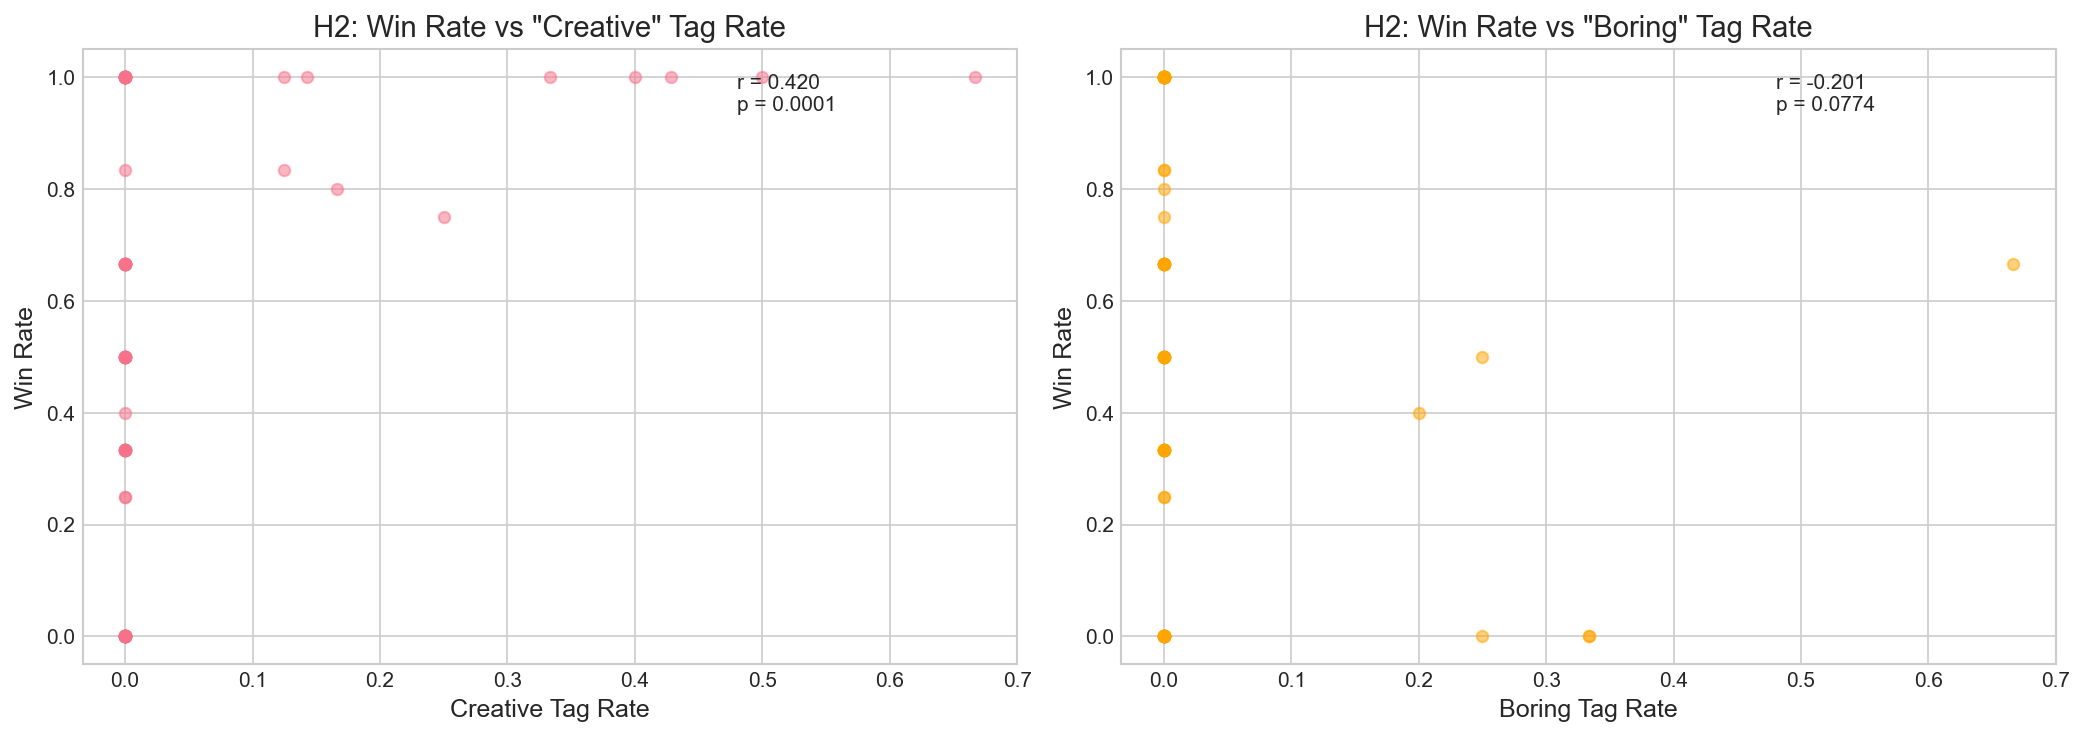
\includegraphics[width=\textwidth]{h2_structural_variety.png}
\end{center}

\column{0.5\textwidth}
\begin{table}
\centering
\footnotesize
\begin{tabular}{lcc}
\toprule
\textbf{Tag} & \textbf{r} & \textbf{p} \\
\midrule
Creative & 0.416 & 0.003 \\
Boring & -0.246 & 0.092 \\
\bottomrule
\end{tabular}
\end{table}

\begin{block}{Conclusion}
Levels tagged ``creative'' win significantly more often.
\end{block}
\end{columns}

\end{frame}

%------------------------------------------------------------
\begin{frame}
\frametitle{RQ1: Path Freedom \& Exploration}

\begin{block}{H3: Agency Hypothesis}
\textbf{Hypothesis:} Levels allowing more exploration are preferred.\\
\textbf{Result:} \alert{Partial Support} -- Backtrack ratio predicts wins ($p=0.019$)
\end{block}

\begin{columns}
\column{0.5\textwidth}
\begin{center}
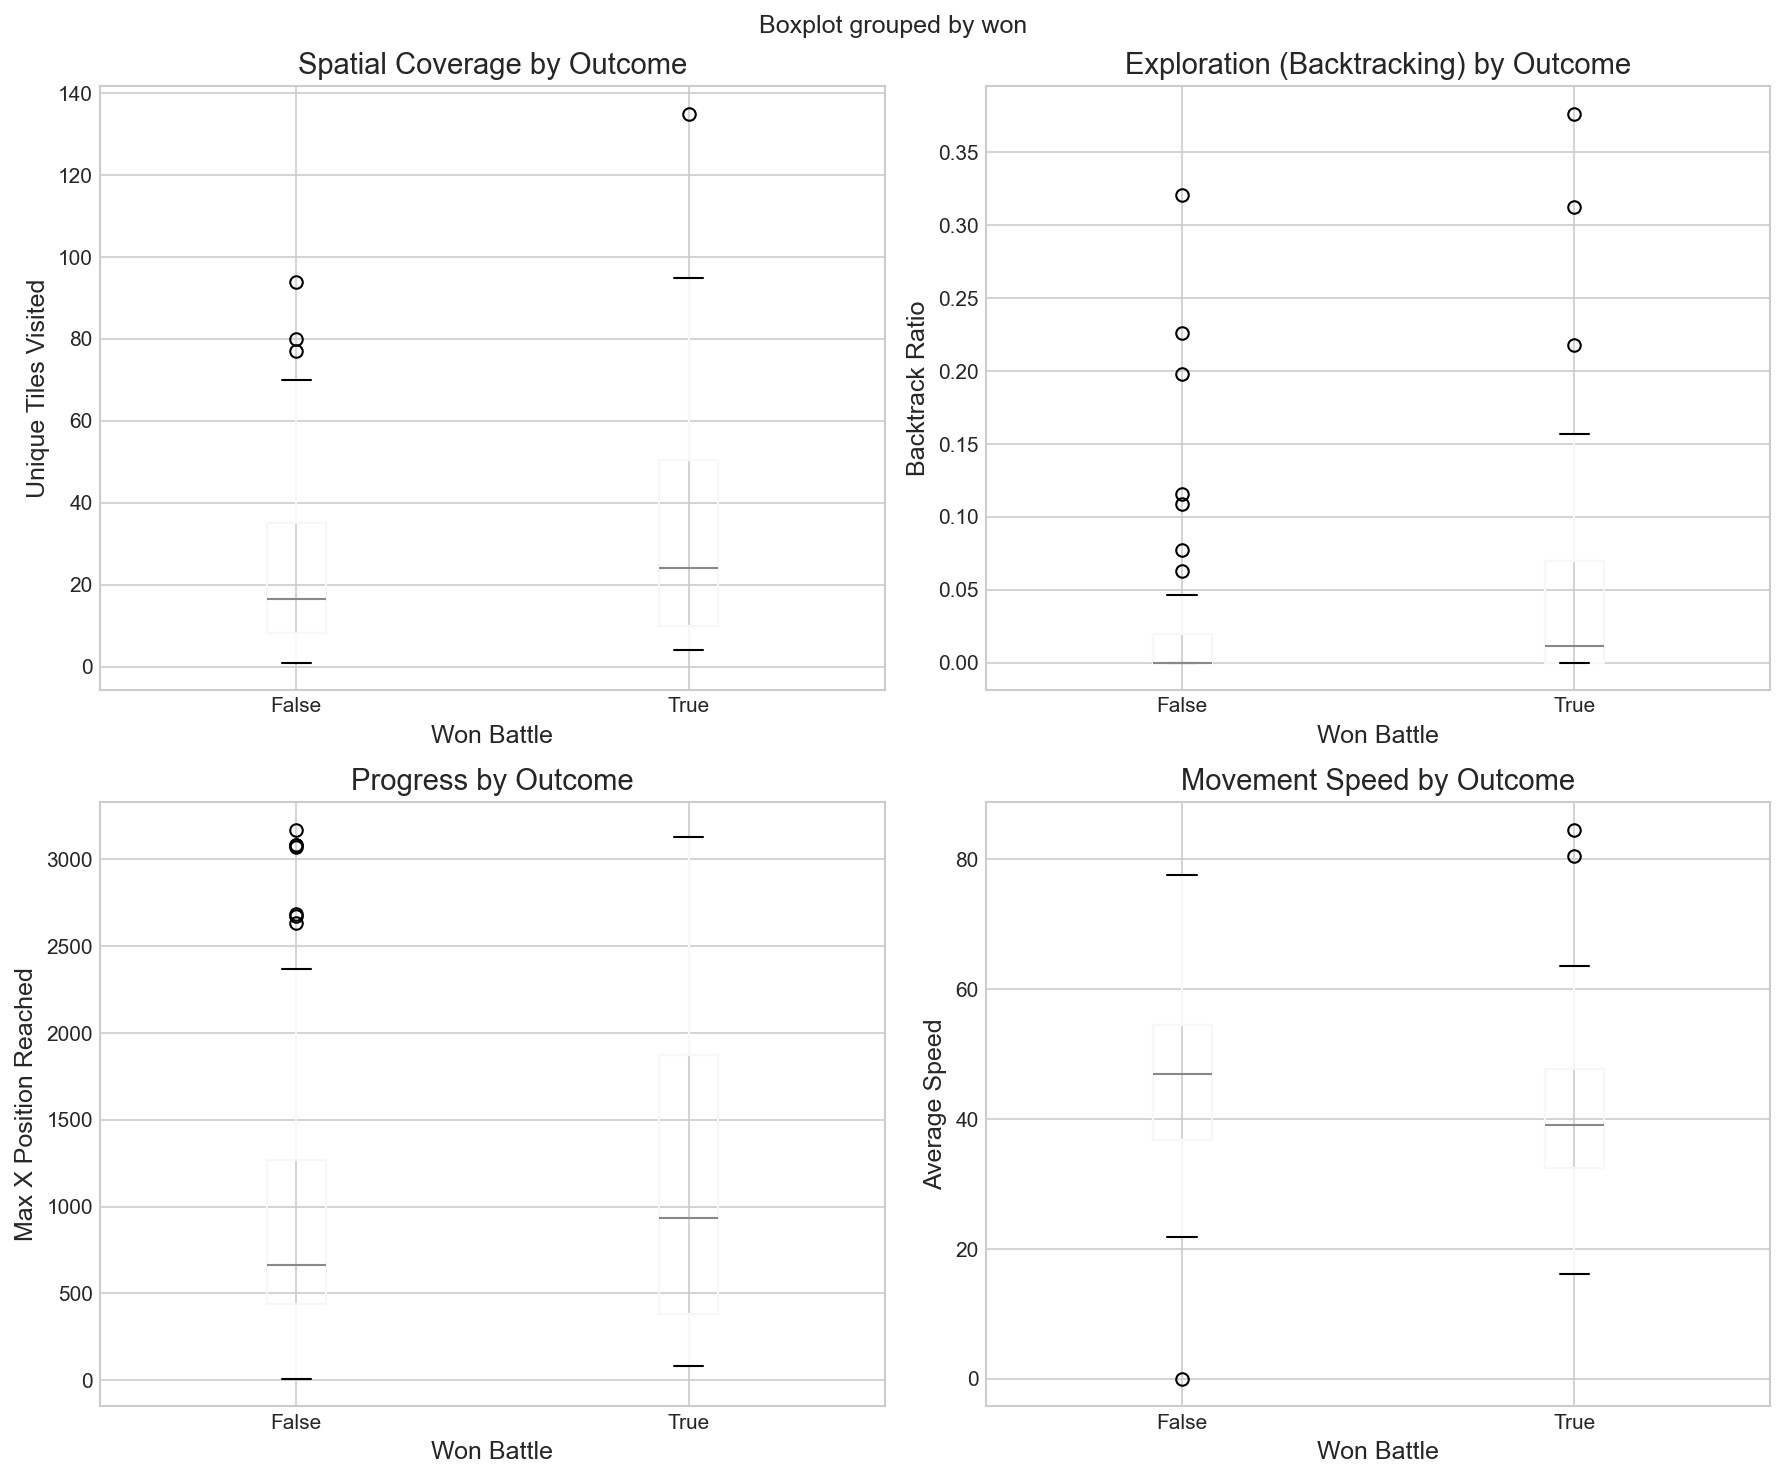
\includegraphics[width=\textwidth]{h3_path_freedom.png}
\end{center}

\column{0.5\textwidth}
\begin{table}
\centering
\footnotesize
\begin{tabular}{lcc}
\toprule
\textbf{Metric} & \textbf{Won} & \textbf{Lost} \\
\midrule
Unique Tiles & 68.7 & 42.1 \\
Backtrack \% & 13\% & 21\% \\
Max X & 1533 & 1095 \\
\bottomrule
\end{tabular}
\end{table}

\begin{block}{Conclusion}
Winners explore \alert{63\% more tiles}. Non-linear paths preferred.
\end{block}
\end{columns}

\end{frame}

%------------------------------------------------------------
\begin{frame}
\frametitle{RQ2: Player Consistency}

\begin{block}{H4: Player Clusters Hypothesis}
\textbf{Hypothesis:} Distinct player preference groups exist.\\
\textbf{Result:} \alert{Supported} -- 3 clusters identified via K-means
\end{block}

\begin{columns}
\column{0.5\textwidth}
\begin{center}
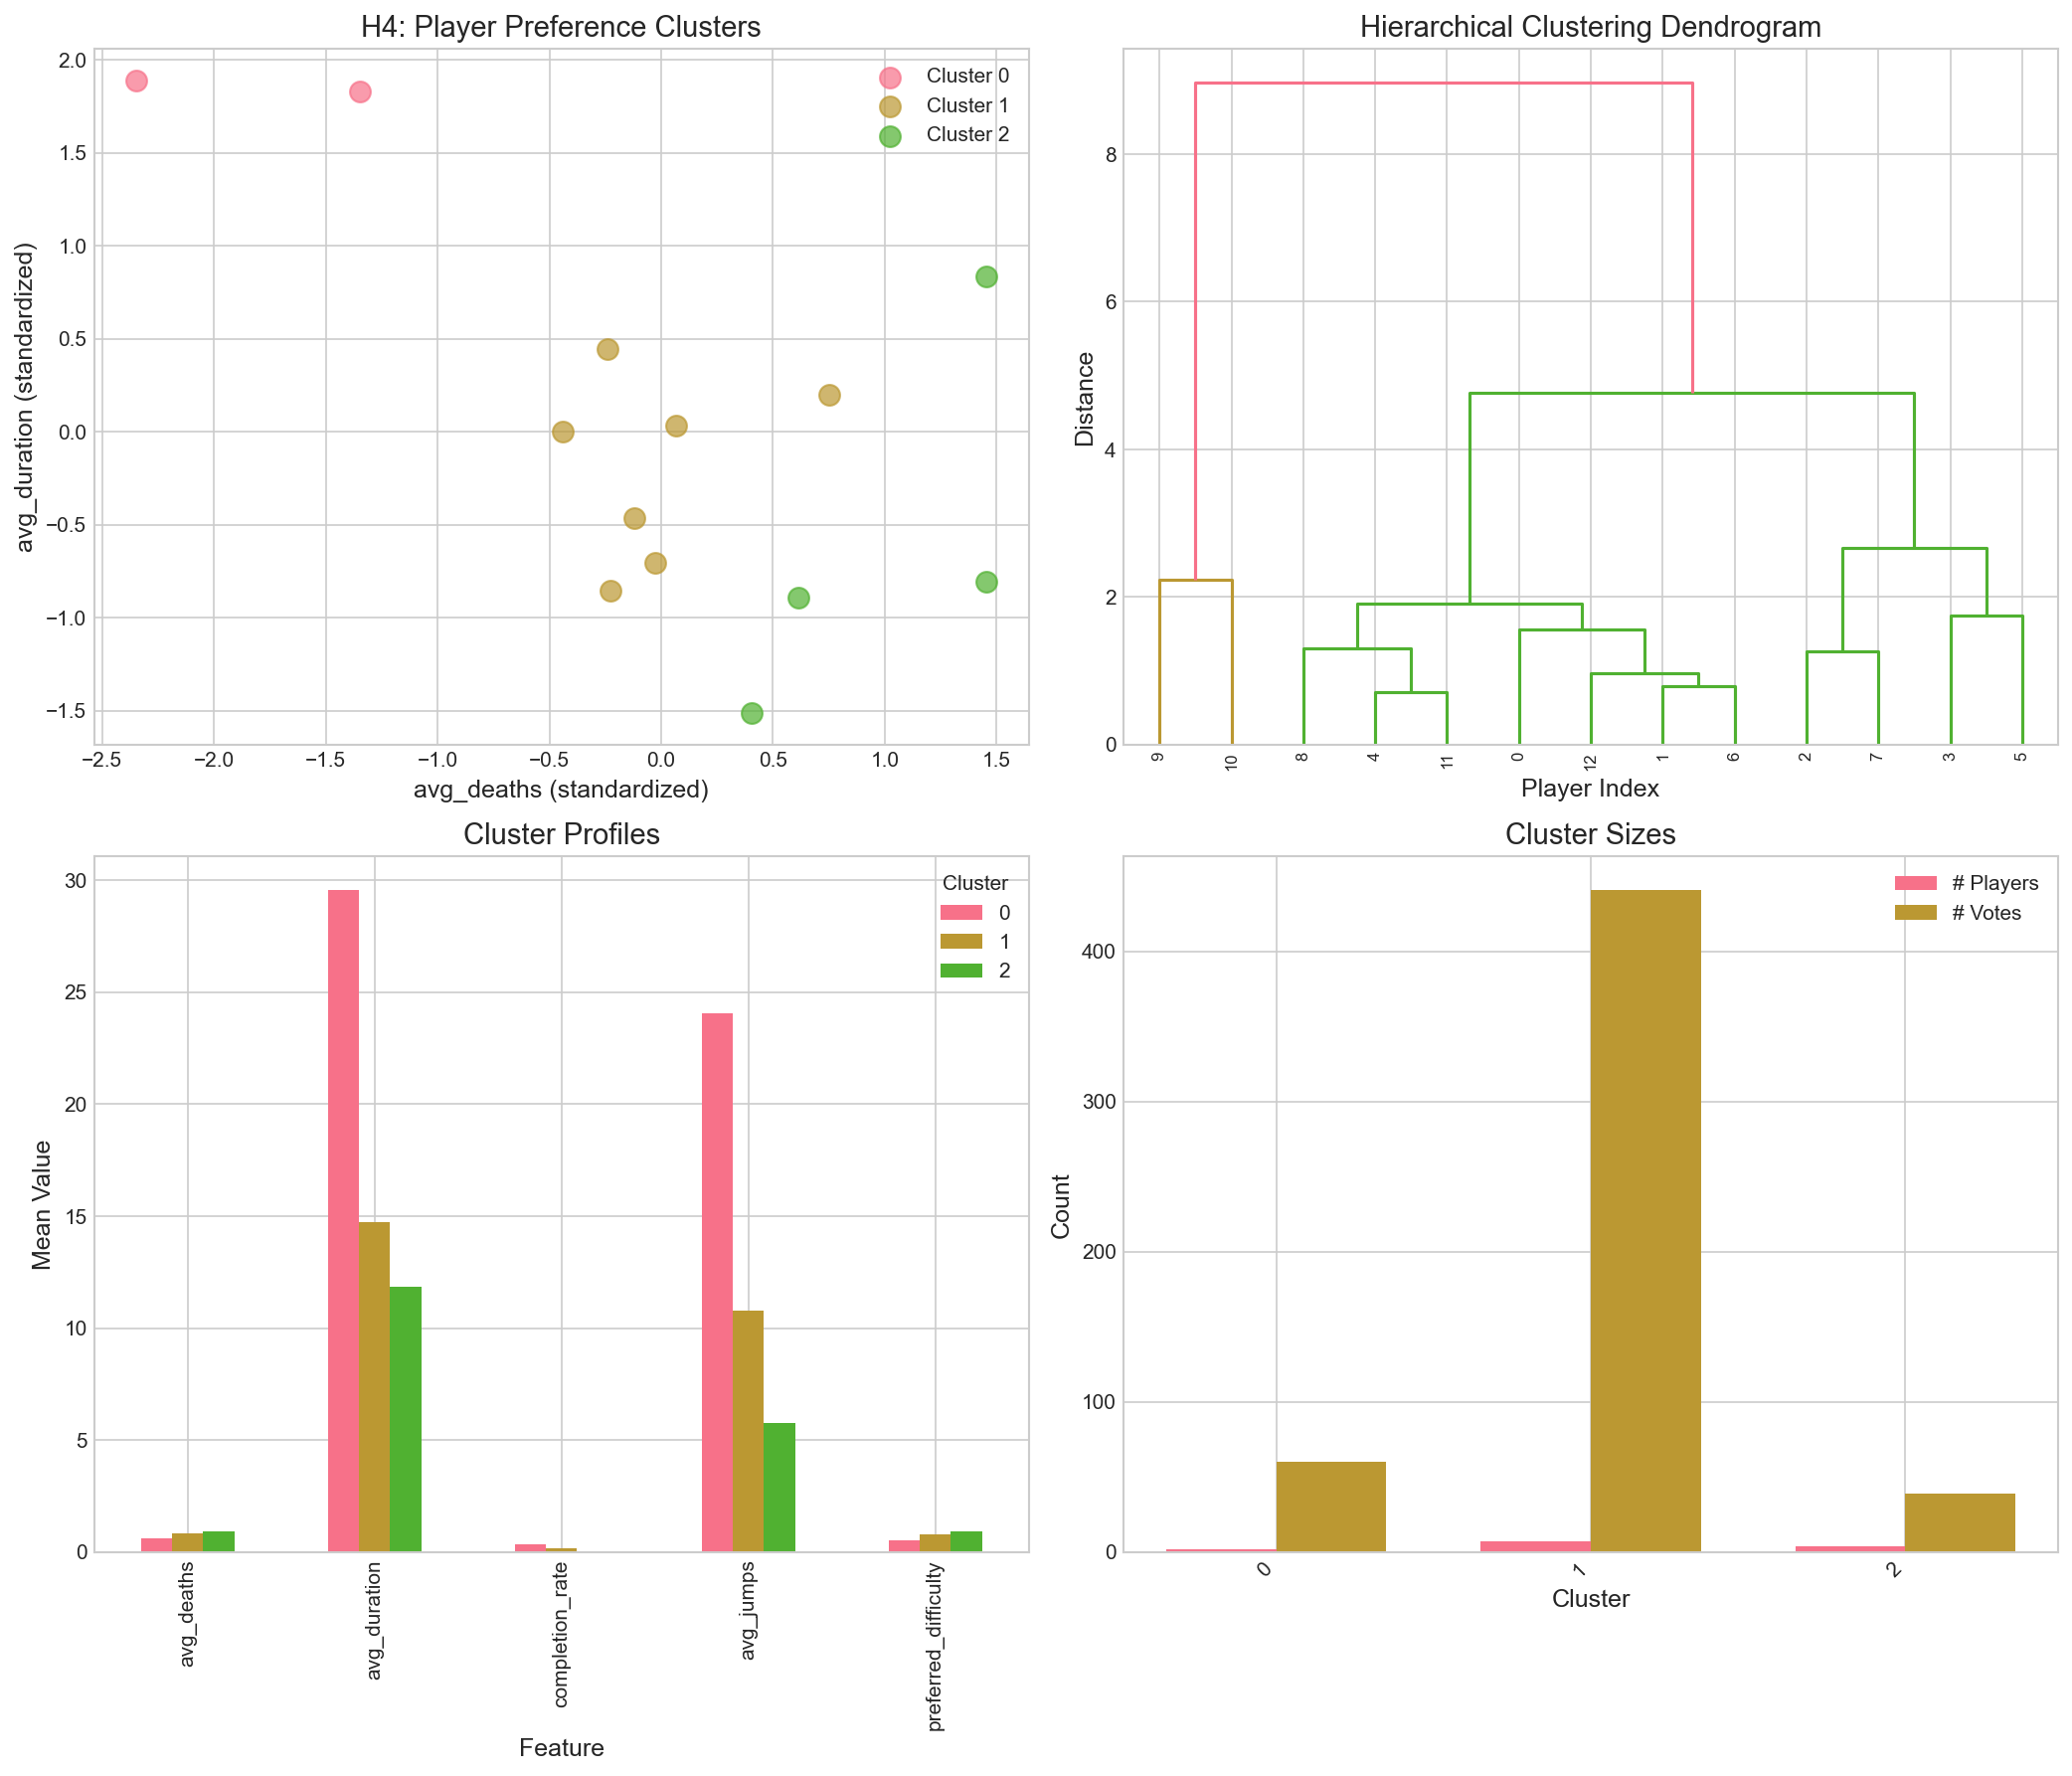
\includegraphics[width=\textwidth]{h4_preference_clusters.png}
\end{center}

\column{0.5\textwidth}
\textbf{Player Types:}
\begin{enumerate}
    \item \textbf{Explorers} (n=2)\\Long sessions, high completion
    \item \textbf{Mainstream} (n=6)\\Most votes, balanced play
    \item \textbf{Strugglers} (n=4)\\Low completion, high deaths
\end{enumerate}
\end{columns}

\end{frame}

%------------------------------------------------------------
\begin{frame}
\frametitle{RQ3: Tag Validation}

\begin{block}{H6: Tags Match Telemetry}
\textbf{Hypothesis:} Subjective tags correlate with objective metrics.\\
\textbf{Result:} \alert{Supported} -- 5/6 tags match expected metric direction
\end{block}

\begin{columns}
\column{0.5\textwidth}
\begin{center}
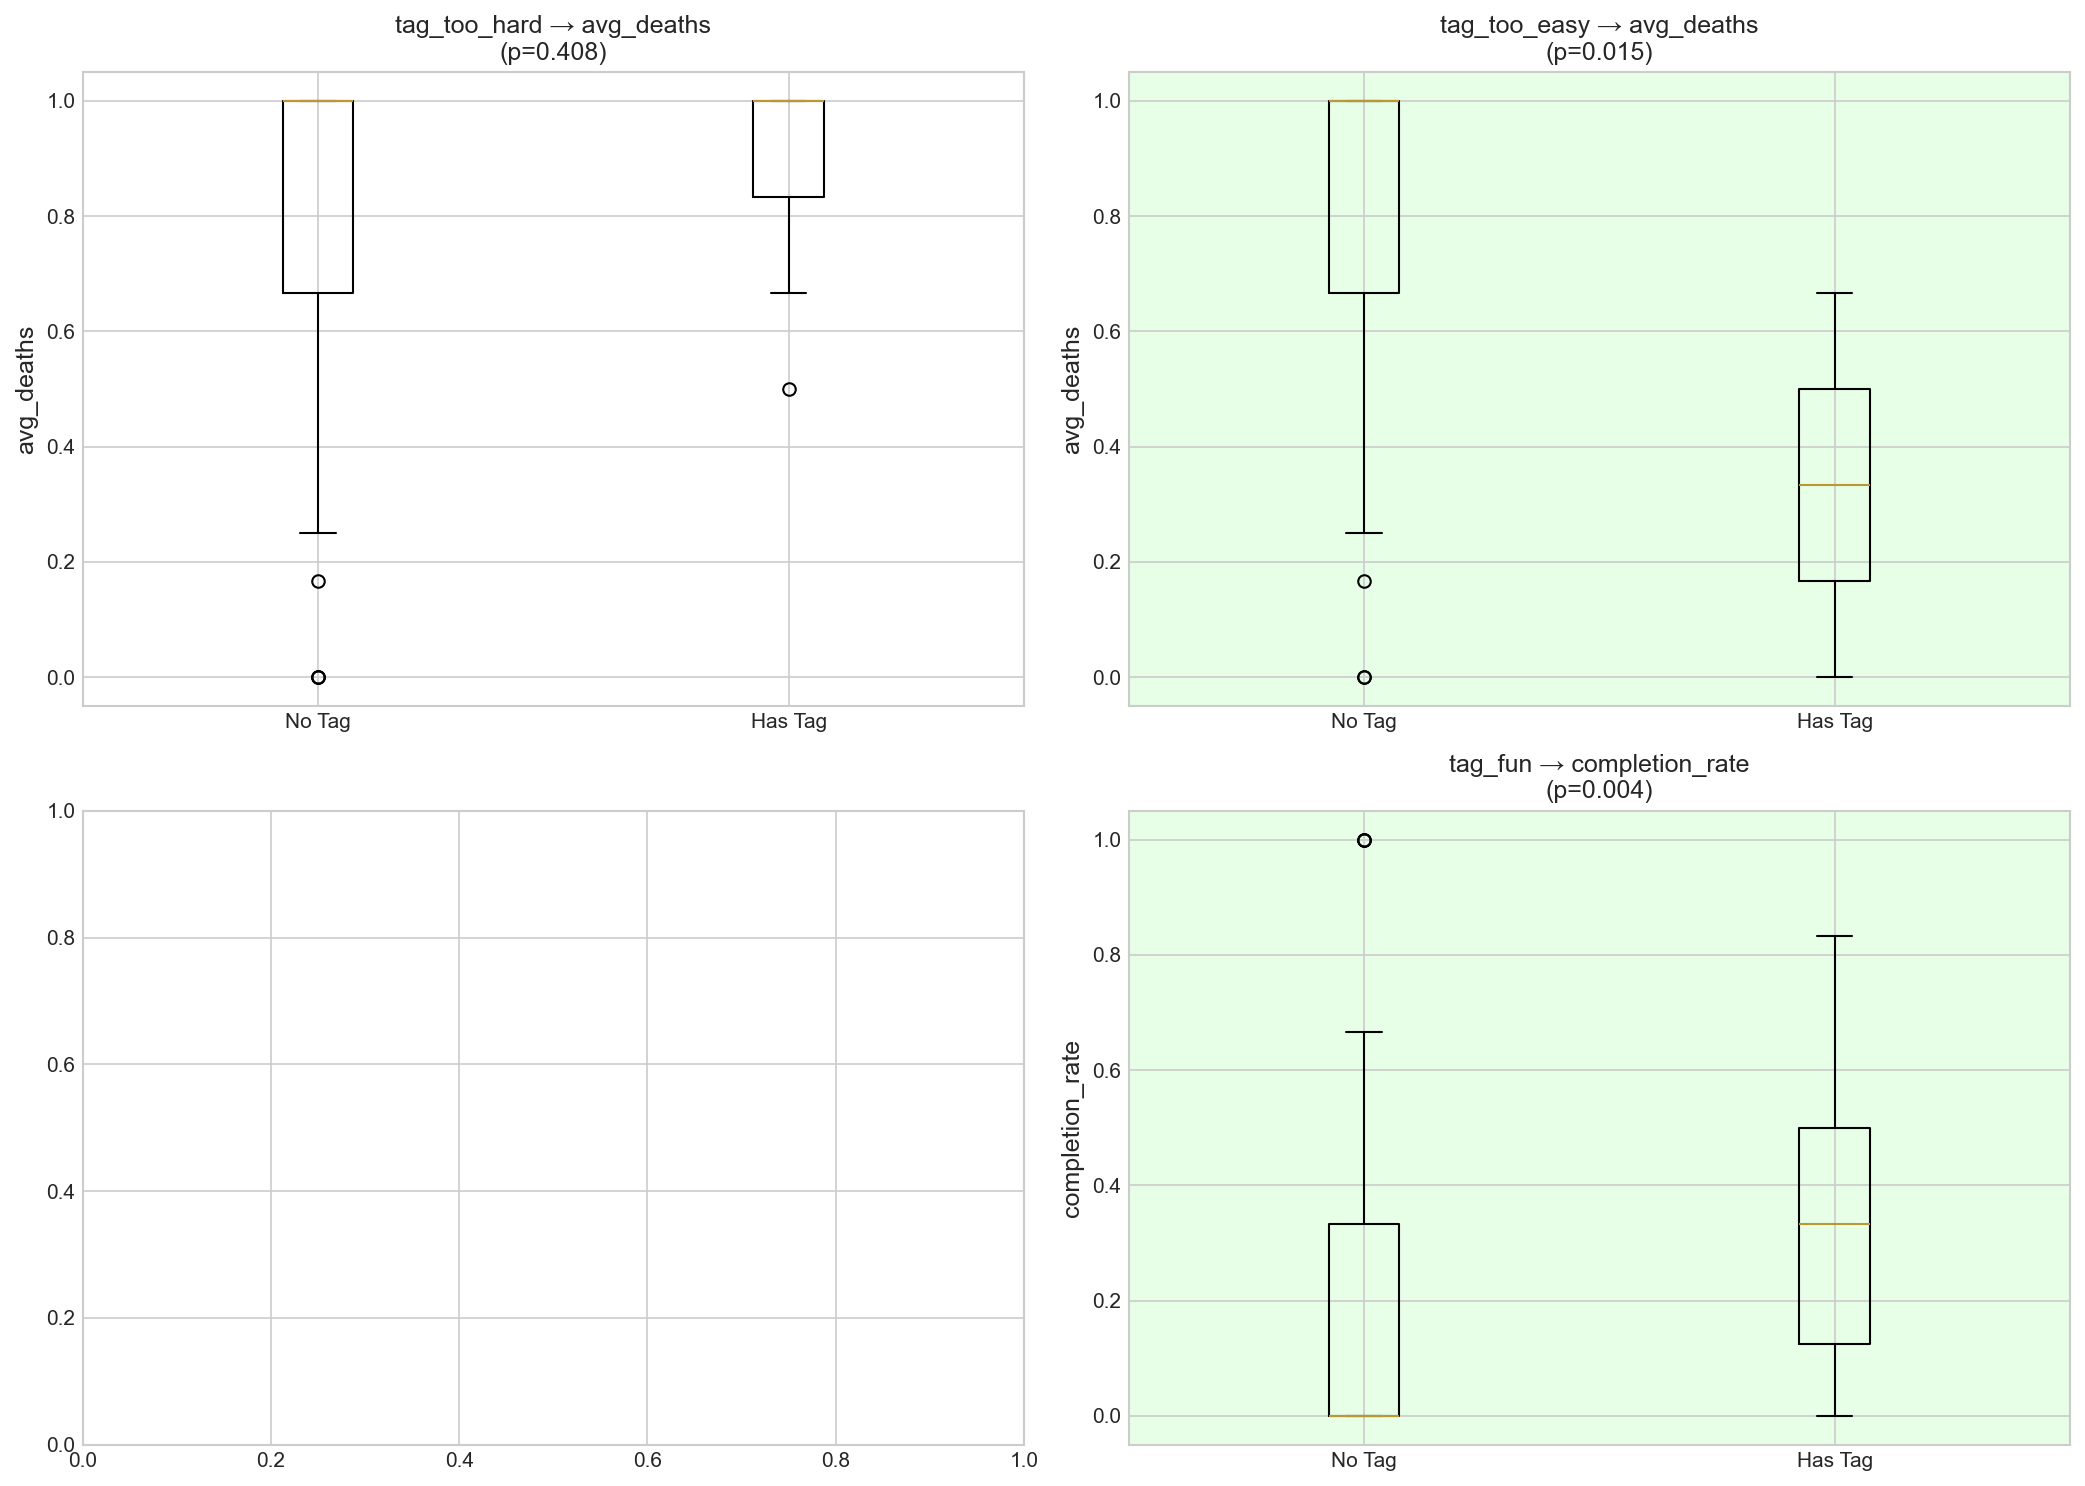
\includegraphics[width=\textwidth]{h6_tag_telemetry.png}
\end{center}

\column{0.5\textwidth}
\textbf{Tag Semantics:}
\begin{itemize}
    \item \texttt{fun} $\approx$ playable + beatable
    \item \texttt{creative} $\approx$ engaging
    \item \texttt{too\_easy} $\approx$ high completion
    \item \texttt{too\_hard} $\approx$ high death rate
\end{itemize}

\begin{block}{Conclusion}
Tags can be \alert{trusted} as quality signals for ML.
\end{block}
\end{columns}

\end{frame}

%==============================================================================
\section{Judge Function \& MarioDPO}
%==============================================================================

%------------------------------------------------------------
\begin{frame}
\frametitle{Building an Automated Judge Function}

\textbf{Goal:} Create reward model for RLHF/DPO training

\vspace{0.5em}
\begin{columns}
\column{0.5\textwidth}
\textbf{Stage 1 -- Static Features:}
$$J_{static} = \frac{w_{style}}{1+D_M} - w_{gap} \cdot \text{Gap}$$

\vspace{0.3em}
\textbf{Stage 2 -- Dynamic Features:}
$$J_{final} = J_{static} + w_{vert} \cdot \sigma_y$$

\column{0.5\textwidth}
\begin{table}
\centering
\footnotesize
\begin{tabular}{lcc}
\toprule
\textbf{Weight} & \textbf{Value} & \textbf{Source} \\
\midrule
$w_{style}$ & 0.32 & Exp D \\
$w_{vert}$ & 0.26 & Exp A \\
$w_{gap}$ & 0.50 & Exp B \\
\bottomrule
\end{tabular}
\end{table}
\end{columns}

\vspace{0.5em}
\begin{alertblock}{Key Result}
Judge function correlates with human preference: \textbf{Spearman $r = 0.812$}, $p < 0.001$
\end{alertblock}

\end{frame}

%------------------------------------------------------------
\begin{frame}
\frametitle{Style Matching: Original Centroid}

\begin{block}{Exp D: Mahalanobis Distance}
\textbf{Hypothesis:} Levels closer to ``Original'' style win more.\\
\textbf{Result:} \alert{Supported} -- $r = -0.279$, $p = 0.011$
\end{block}

\begin{columns}
\column{0.5\textwidth}
\begin{center}
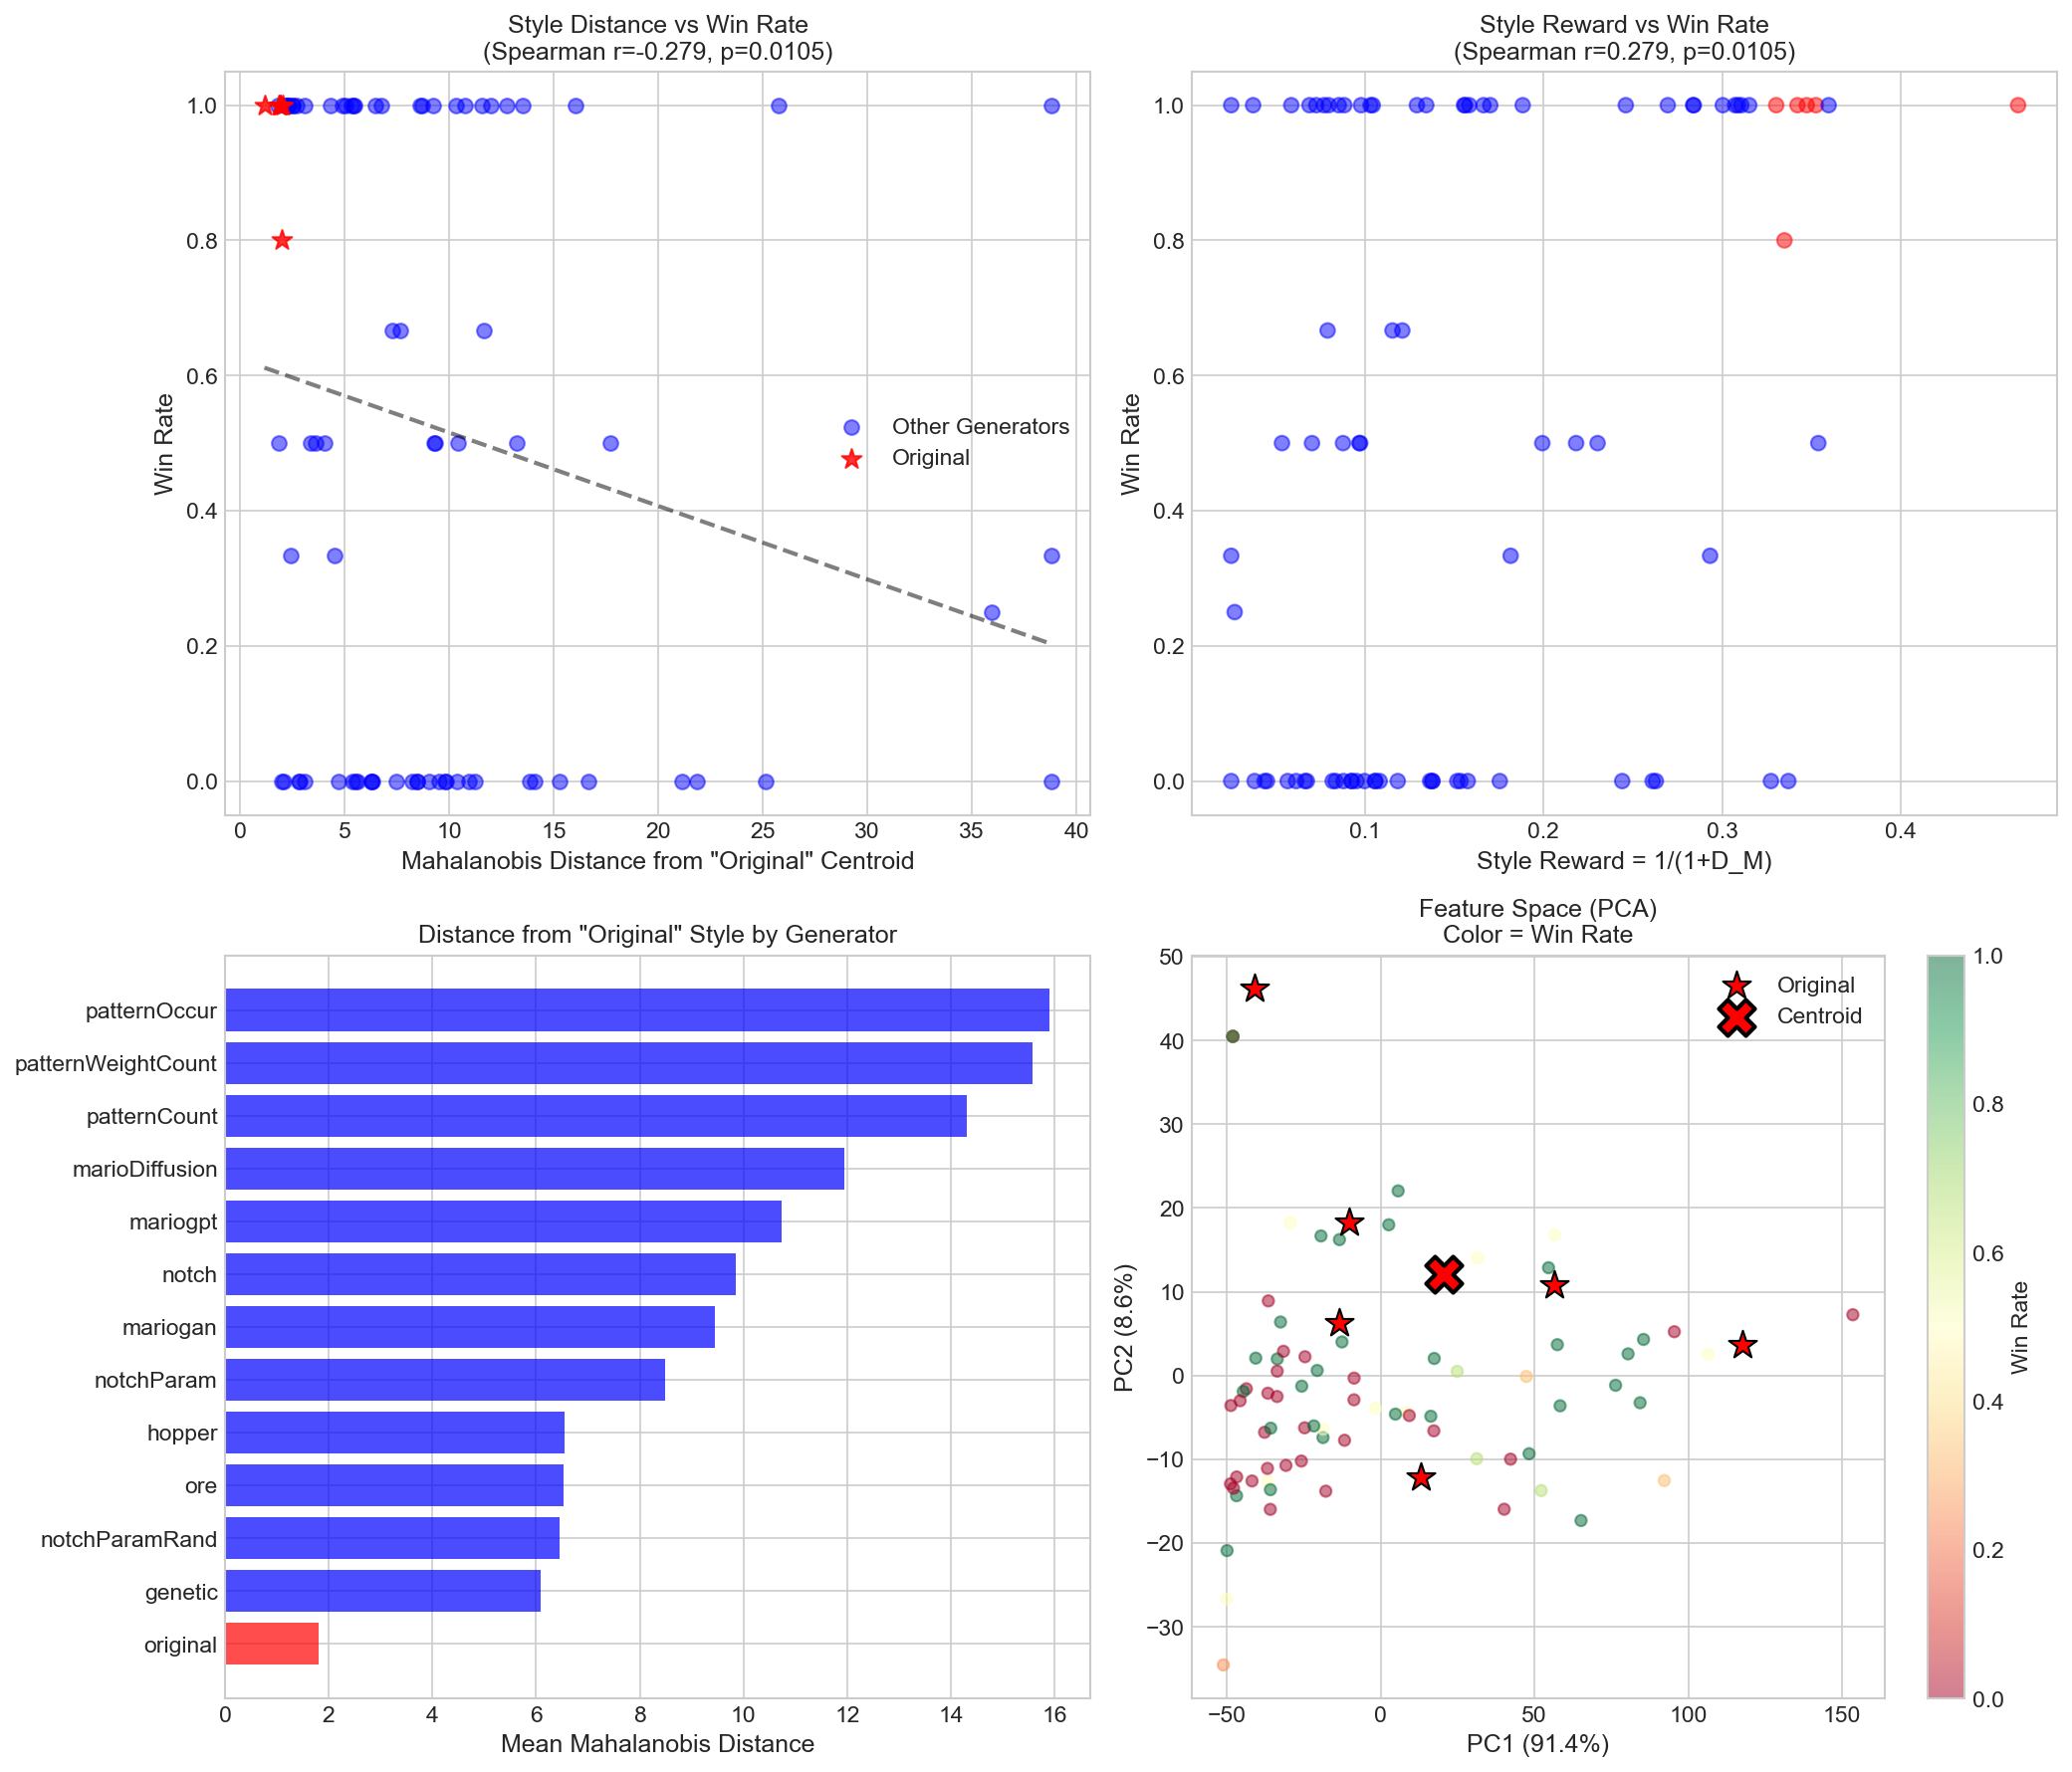
\includegraphics[width=\textwidth]{exp_d_original_centroid.png}
\end{center}

\column{0.5\textwidth}
\begin{block}{Conclusion}
The ``Nintendo Factor'': original SMB levels define the \alert{quality target}.

\vspace{0.3em}
Style reward:
$$r_{style} = \frac{1}{1 + D_M}$$

where $D_M$ = Mahalanobis distance
\end{block}
\end{columns}

\end{frame}

%------------------------------------------------------------
\begin{frame}
\frametitle{MarioDPO: Aligning Generators with Human Preferences}

\textbf{Approach:} Direct Preference Optimization (DPO) fine-tuning

\begin{columns}
\column{0.5\textwidth}
\begin{block}{Training Data}
\begin{itemize}
    \item 571 human pairs ($\times$10 weight)
    \item 3,500+ synthetic pairs (Judge)
    \item \textbf{9,200+ effective pairs}
\end{itemize}
\end{block}

\begin{block}{Architecture}
\begin{itemize}
    \item Base: GPT-2 small
    \item Tokenization: Character-level
    \item DPO $\beta = 0.1$
\end{itemize}
\end{block}

\column{0.5\textwidth}
\begin{center}
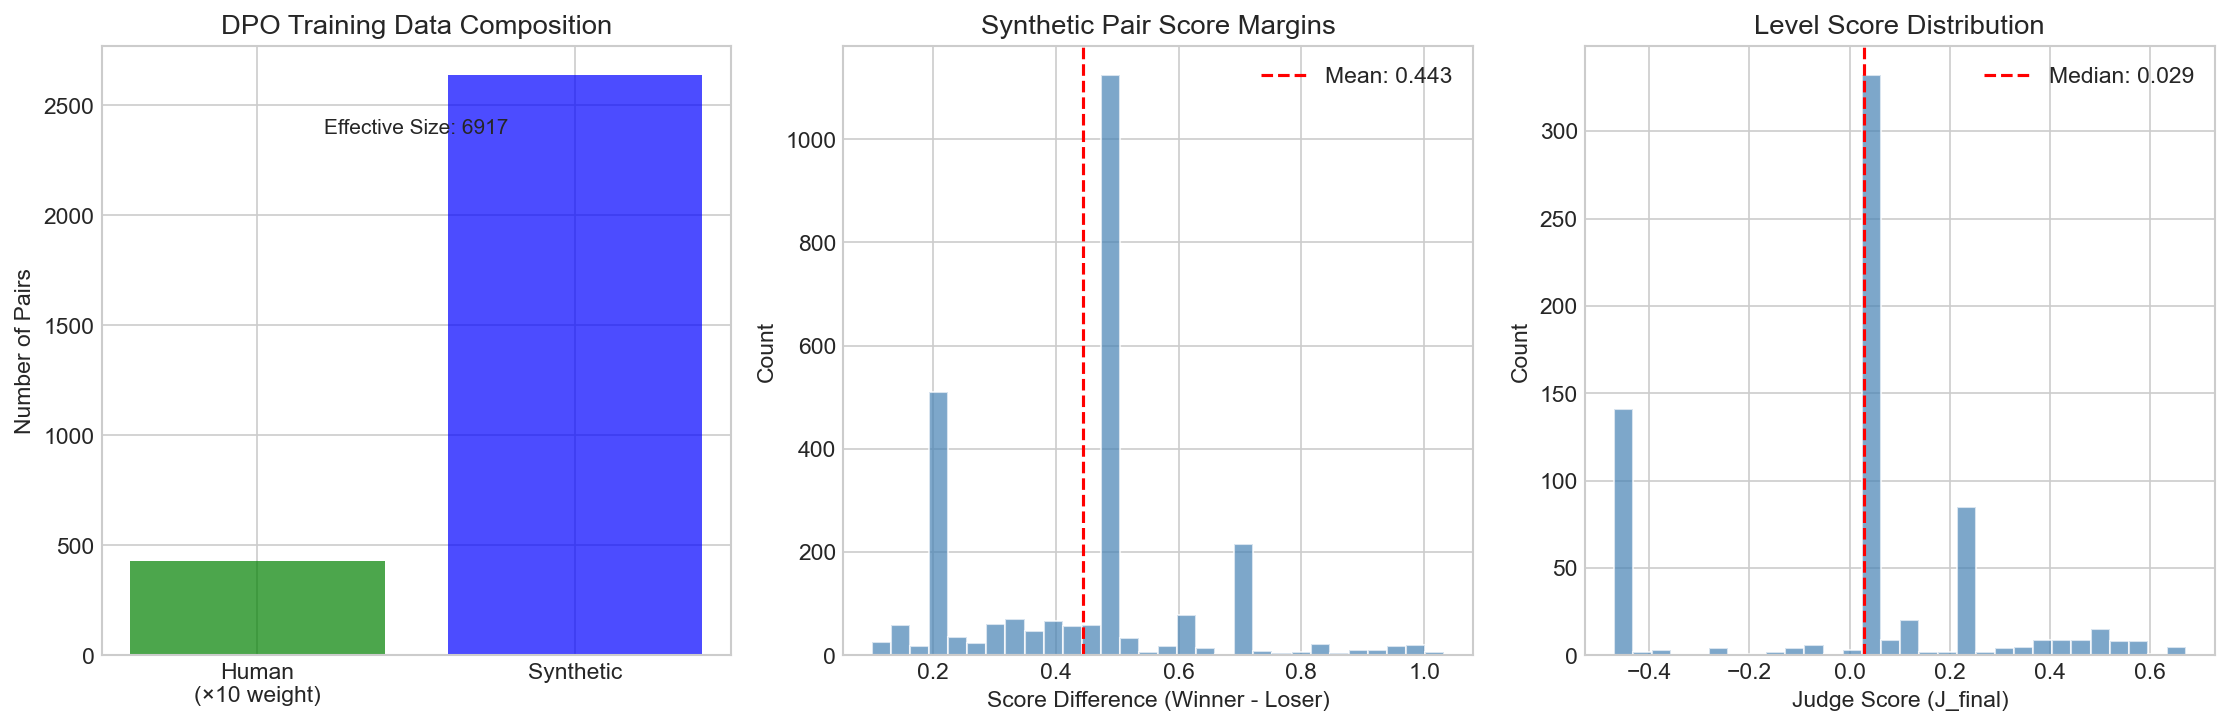
\includegraphics[width=\textwidth]{dpo_training_data.png}
\end{center}
\end{columns}

\end{frame}

%------------------------------------------------------------
\begin{frame}
\frametitle{MarioDPO Results: Beating Other PCG Methods}

\begin{center}
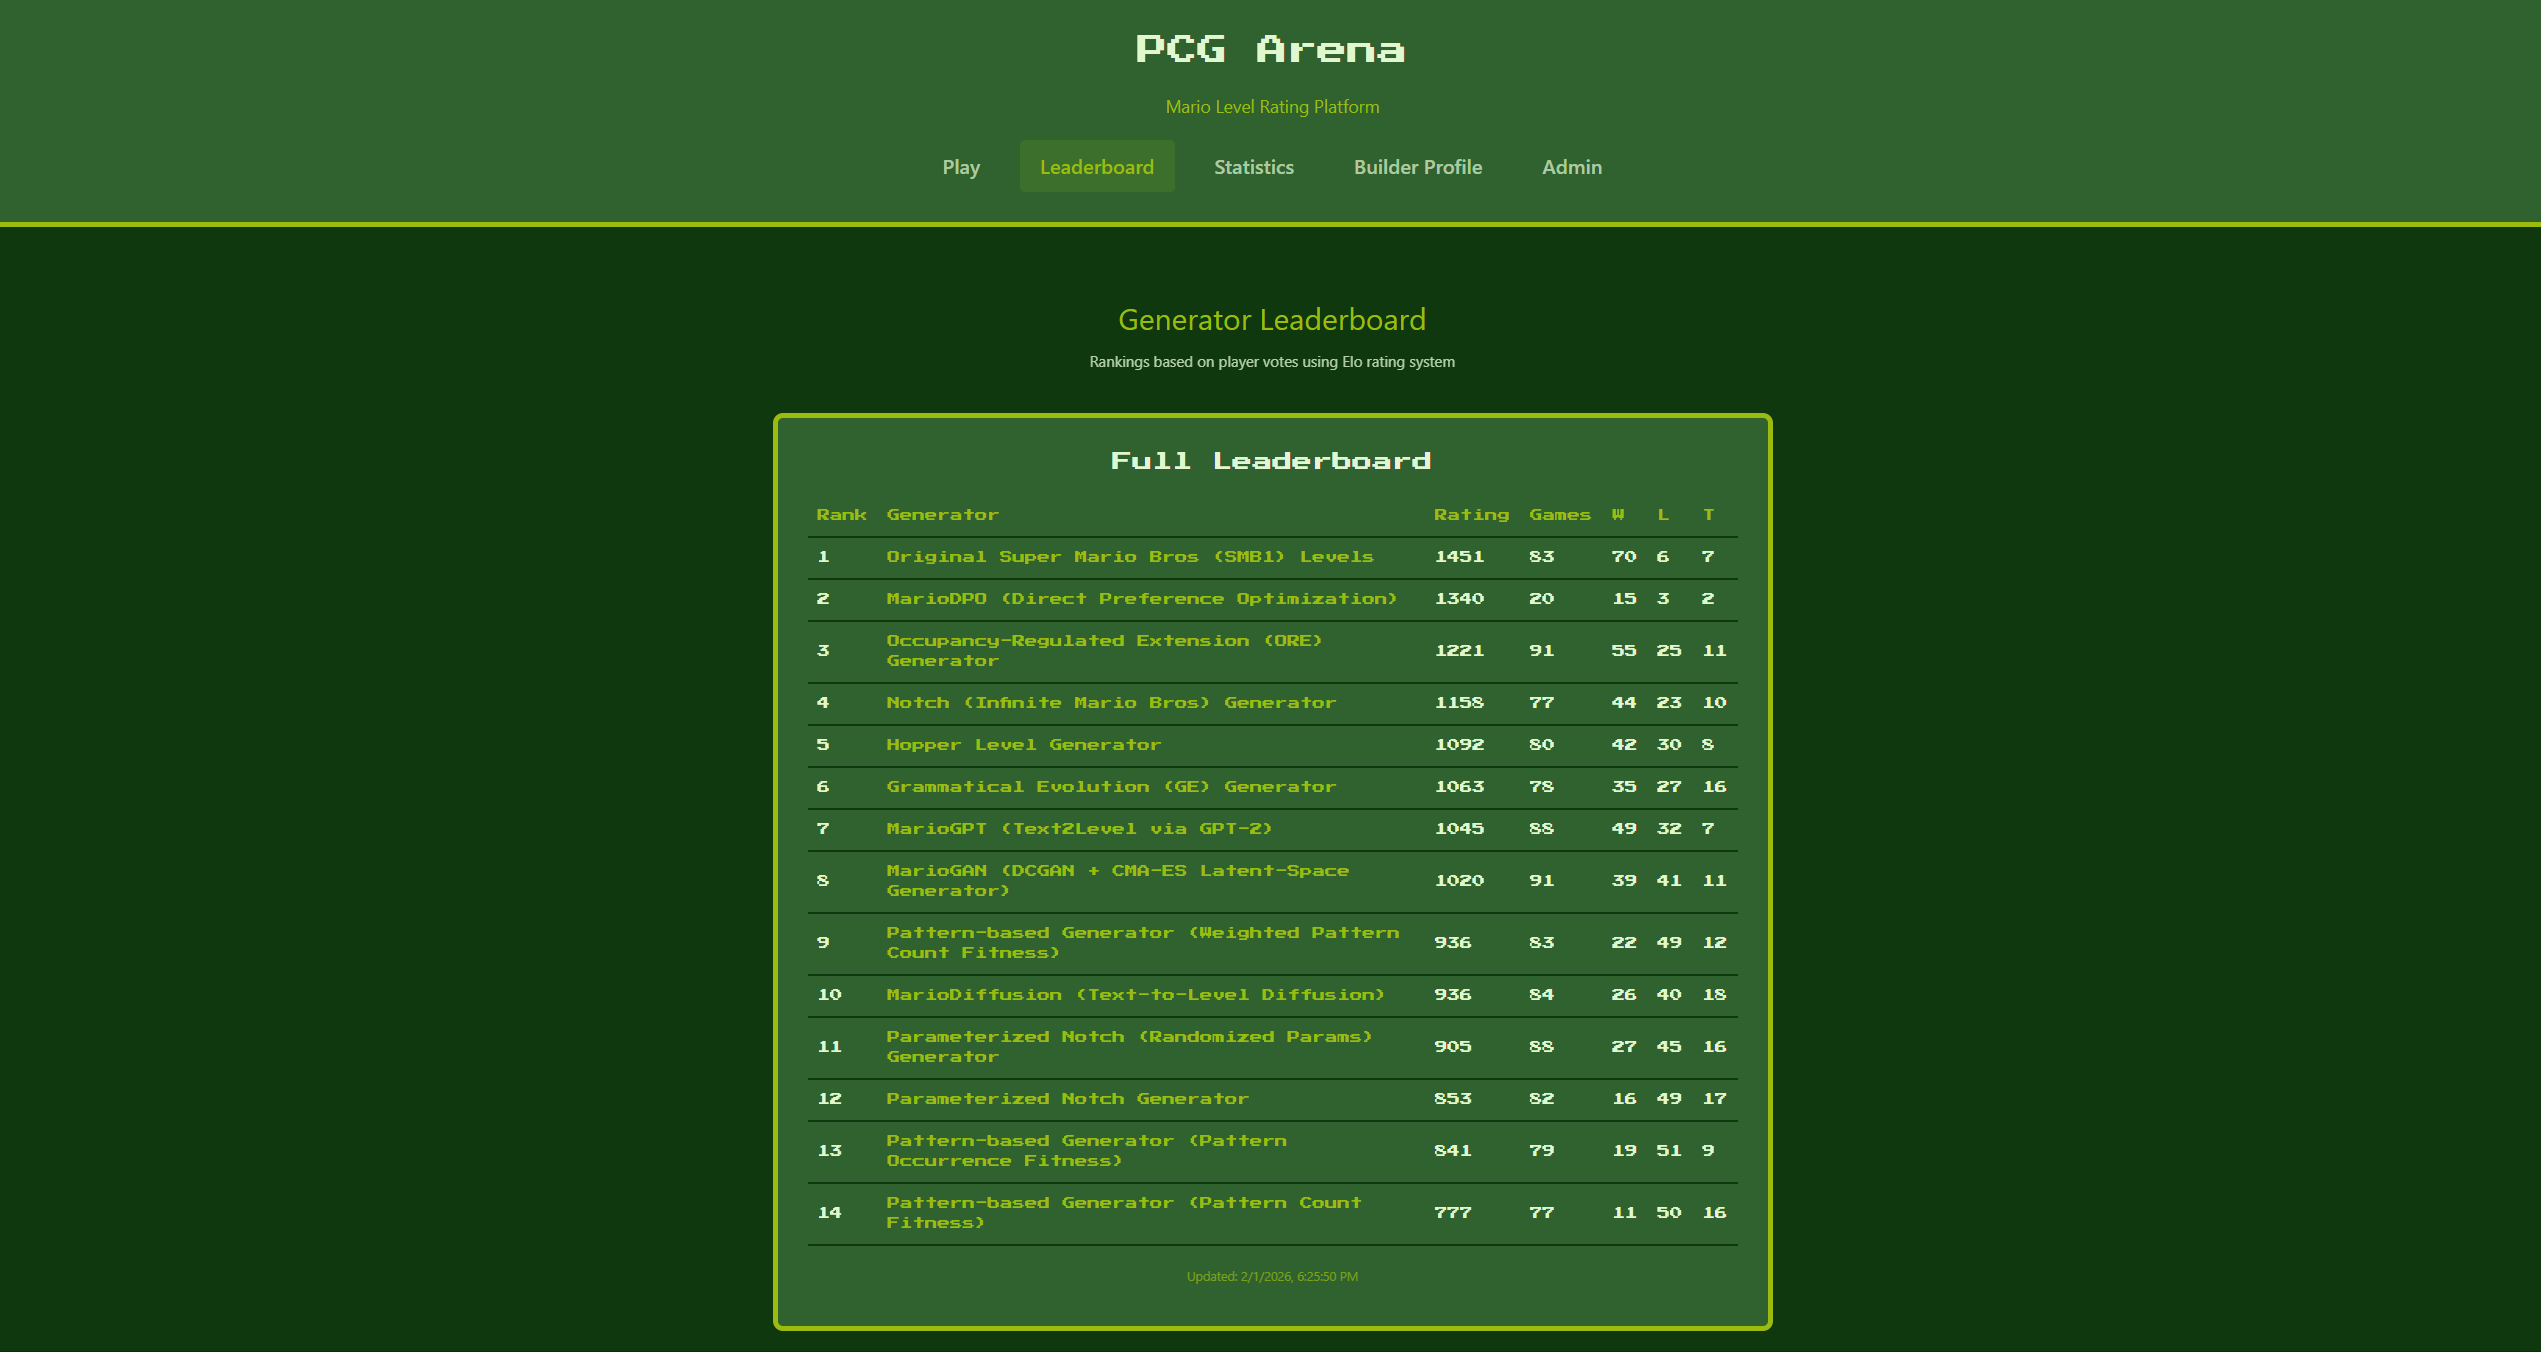
\includegraphics[width=0.85\textwidth]{MarioDPO_better_than_other_pcg.png}
\end{center}

\vspace{-0.5em}
\begin{alertblock}{Key Achievement}
\textbf{MarioDPO achieves highest Elo among all PCG generators}, second only to hand-crafted Original SMB levels!
\end{alertblock}

\end{frame}

%------------------------------------------------------------
\begin{frame}
\frametitle{Generator Rankings Summary}

\begin{columns}
\column{0.55\textwidth}
\begin{table}
\centering
\footnotesize
\begin{tabular}{clc}
\toprule
\textbf{Rank} & \textbf{Generator} & \textbf{Win Rate} \\
\midrule
1 & \textbf{Original (SMB)} & 89.6\% \\
2 & \alert{MarioDPO (ours)} & \alert{83.3\%} \\
3 & ORE & 69.3\% \\
4 & Notch & 67.4\% \\
5 & MarioGPT & 63.8\% \\
\midrule
12 & patternOccur & 26.1\% \\
13 & notchParam & 23.9\% \\
14 & patternCount & 20.4\% \\
\bottomrule
\end{tabular}
\end{table}

\column{0.45\textwidth}
\begin{block}{Key Insights}
\begin{itemize}
    \item Original dominates (89\%)
    \item \alert{MarioDPO} beats other ML methods
    \item Pattern generators fail
    \item Style distance predicts quality
\end{itemize}
\end{block}
\end{columns}

\end{frame}

%==============================================================================
\section{Conclusions}
%==============================================================================

%------------------------------------------------------------
\begin{frame}
\frametitle{Key Findings}

\begin{enumerate}
    \item \textbf{Playability $>$ Challenge}\\
    Players prefer levels they can complete (no flow channel)
    
    \vspace{0.5em}
    \item \textbf{Exploration Matters}\\
    Non-linear, explorable levels win 63\% more tiles visited
    
    \vspace{0.5em}
    \item \textbf{Style Matching Works}\\
    Closer to Original SMB $\rightarrow$ higher win rate ($r = 0.28$)
    
    \vspace{0.5em}
    \item \textbf{Tags are Valid Signals}\\
    Subjective tags correlate with objective metrics (5/6)
    
    \vspace{0.5em}
    \item \textbf{DPO Alignment Succeeds}\\
    MarioDPO achieves \alert{highest Elo} among PCG generators
\end{enumerate}

\end{frame}

%------------------------------------------------------------
\begin{frame}
\frametitle{Contributions}

\begin{block}{Platform}
\begin{itemize}
    \item Open-source web platform for PCG evaluation
    \item Mario engine ported Java $\rightarrow$ TypeScript
    \item Glicko-2 + AGIS matchmaking
\end{itemize}
\end{block}

\begin{block}{Research}
\begin{itemize}
    \item Empirical comparison of 15 generators
    \item Validated judge function ($r = 0.28$)
    \item MarioDPO: SOTA among PCG methods (83.3\%)
\end{itemize}
\end{block}

\begin{block}{Data}
\begin{itemize}
    \item 748 levels, 571 human votes
    \item Player trajectories and death heatmaps
    \item Open dataset for future research
\end{itemize}
\end{block}

\end{frame}

%------------------------------------------------------------
\begin{frame}
\frametitle{Future Work}

\begin{columns}
\column{0.5\textwidth}
\textbf{Short-term}
\begin{itemize}
    \item Collect more votes
    \item Add more generators
    \item Improve matchmaking
\end{itemize}

\column{0.5\textwidth}
\textbf{Long-term}
\begin{itemize}
    \item Transfer to other games
    \item Online DPO training
    \item Multi-objective PCG
\end{itemize}
\end{columns}

\vspace{1em}
\begin{center}
\Large
\alert{\url{https://pcg-arena.com}}

\vspace{0.5em}
\normalsize
Try it yourself!
\end{center}

\end{frame}

%------------------------------------------------------------
\begin{frame}
\frametitle{Thank You!}

\begin{center}
\Large
\textbf{Questions?}

\vspace{2em}
\normalsize
\begin{tabular}{ll}
\textbf{Platform:} & \url{https://pcg-arena.com} \\
\textbf{Code:} & \url{https://github.com/antoniczapski/pcg-arena} \\
\end{tabular}

\vspace{2em}
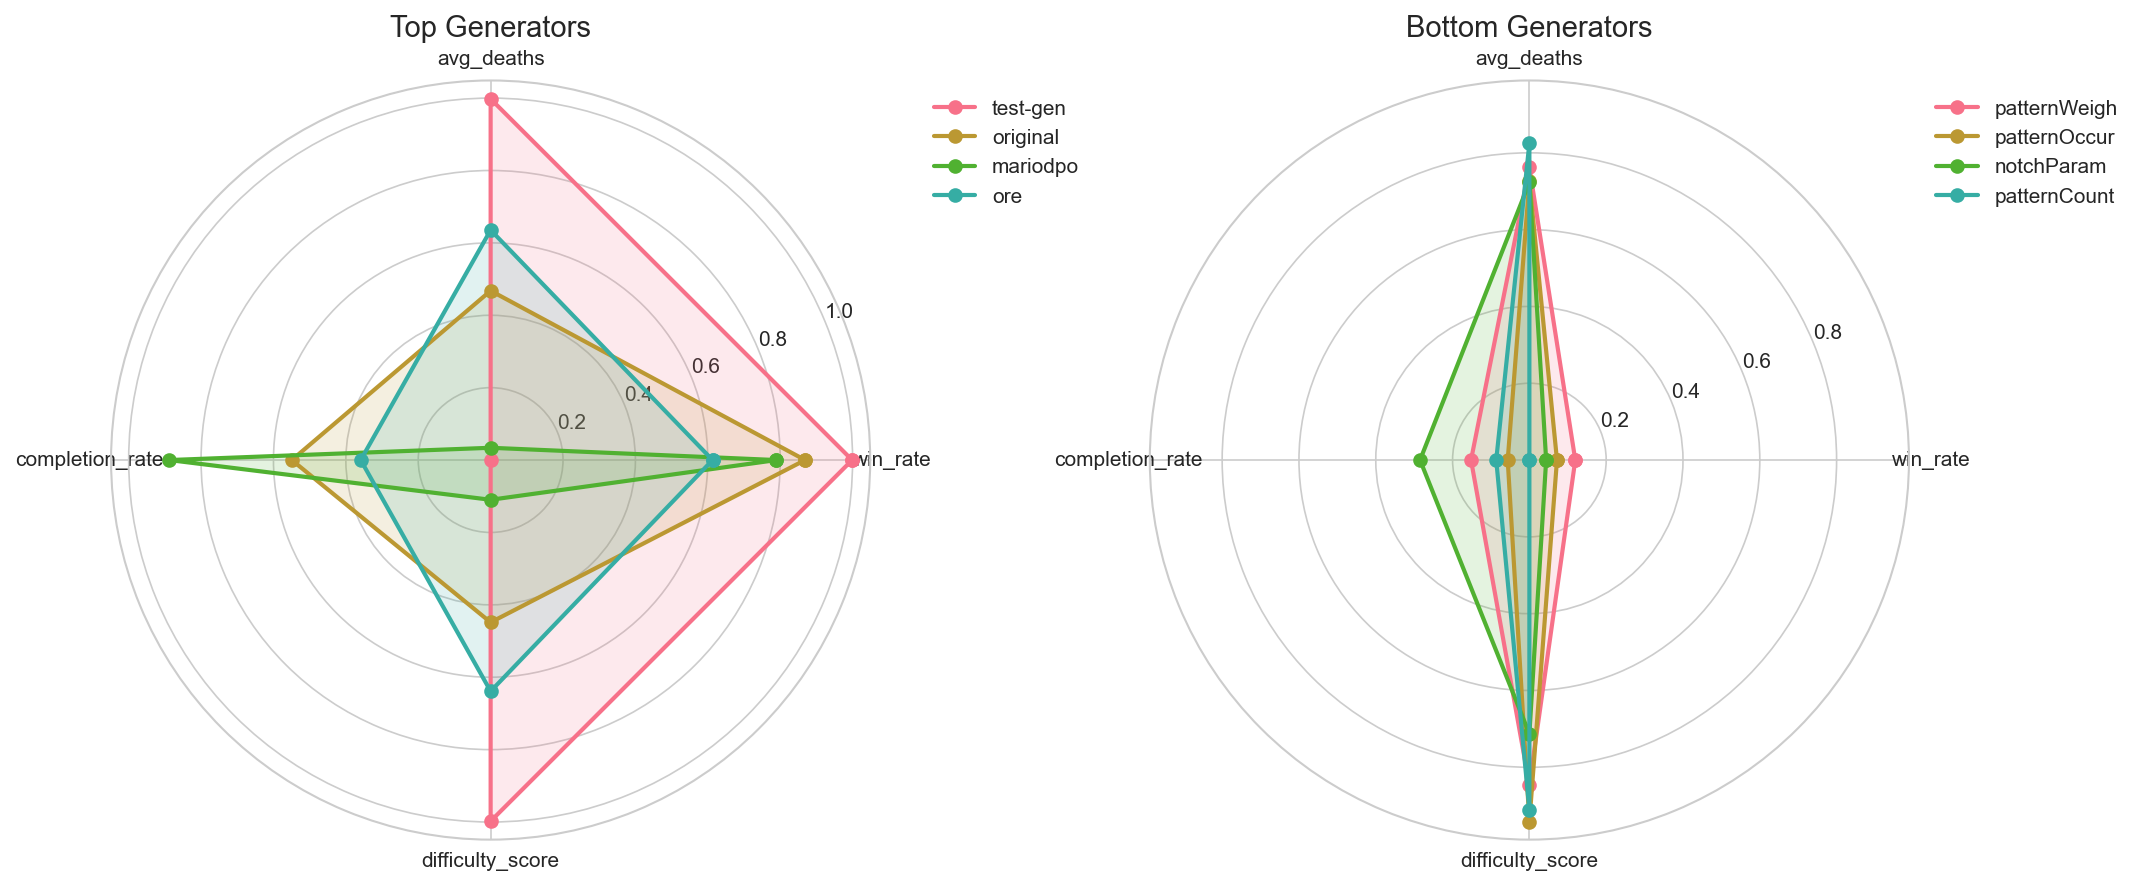
\includegraphics[width=0.3\textwidth]{generator_fingerprints.png}
\end{center}

\end{frame}

%==============================================================================
% Backup slides
%==============================================================================

\appendix

\begin{frame}
\frametitle{Backup: Generator Fingerprints}
\begin{center}
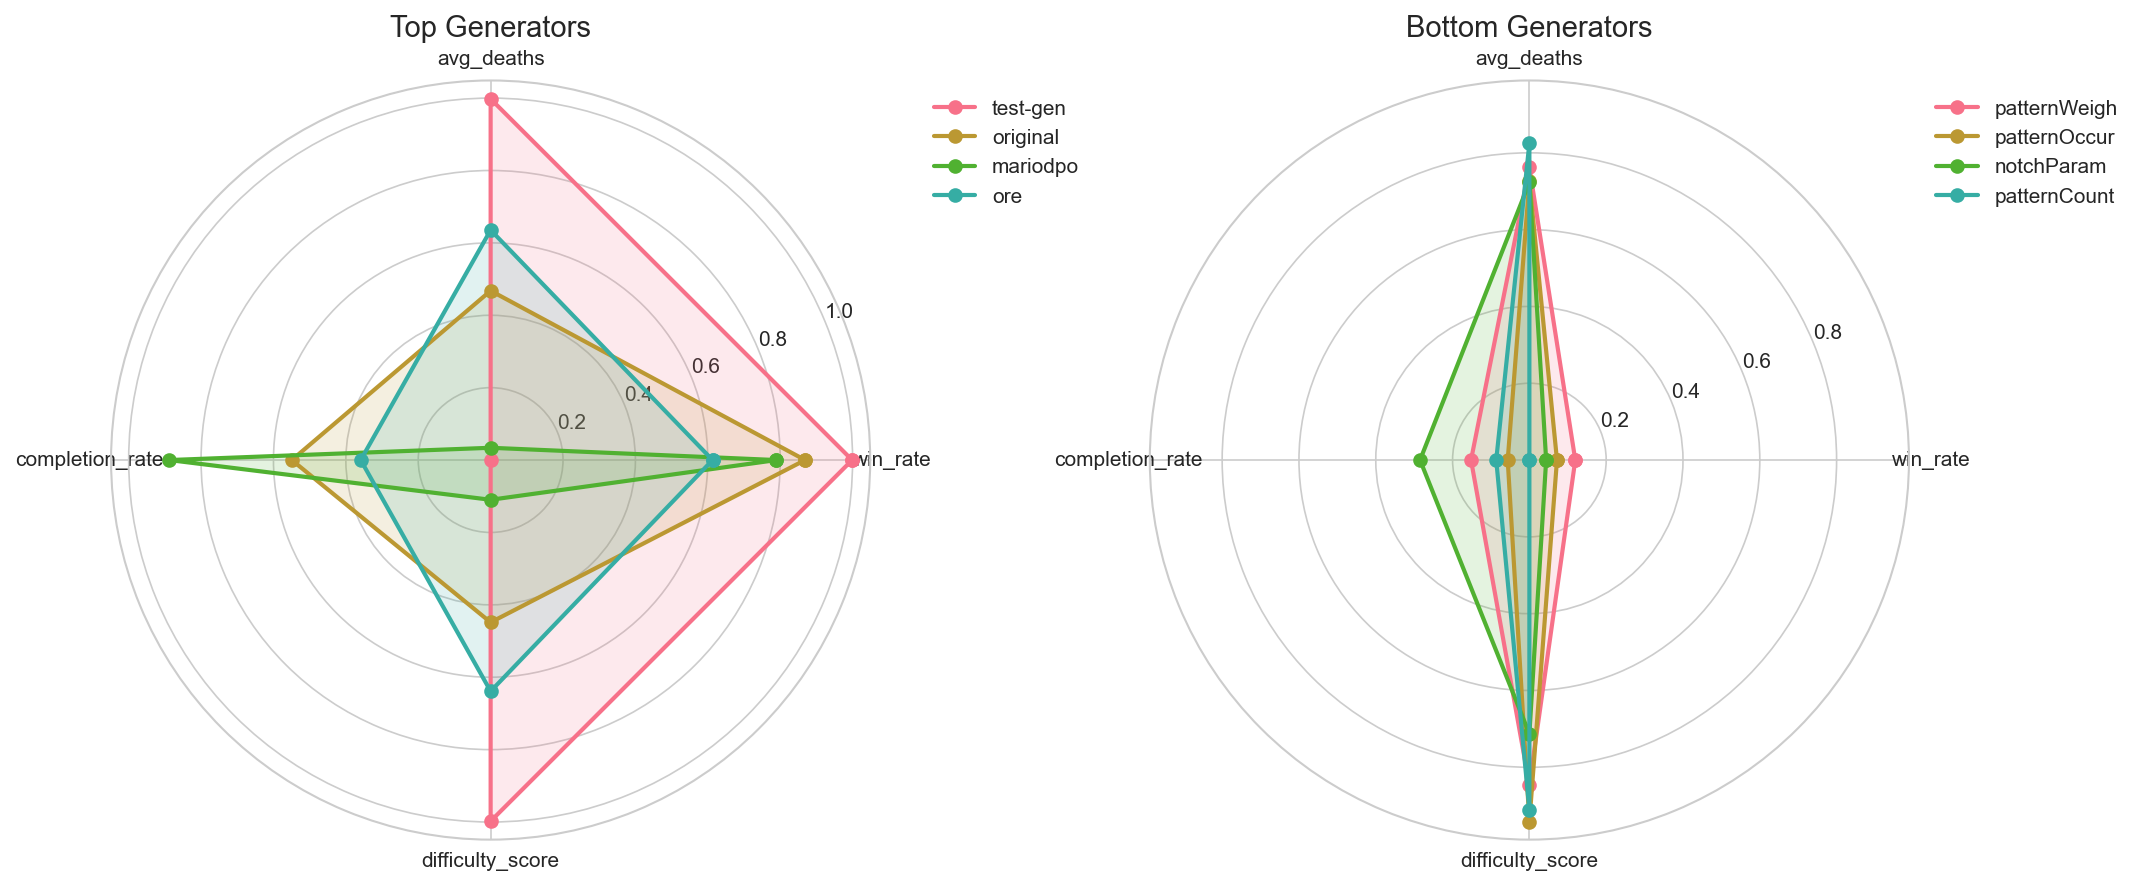
\includegraphics[width=0.9\textwidth]{generator_fingerprints.png}
\end{center}
\end{frame}

\begin{frame}
\frametitle{Backup: Correlation Matrix}
\begin{center}
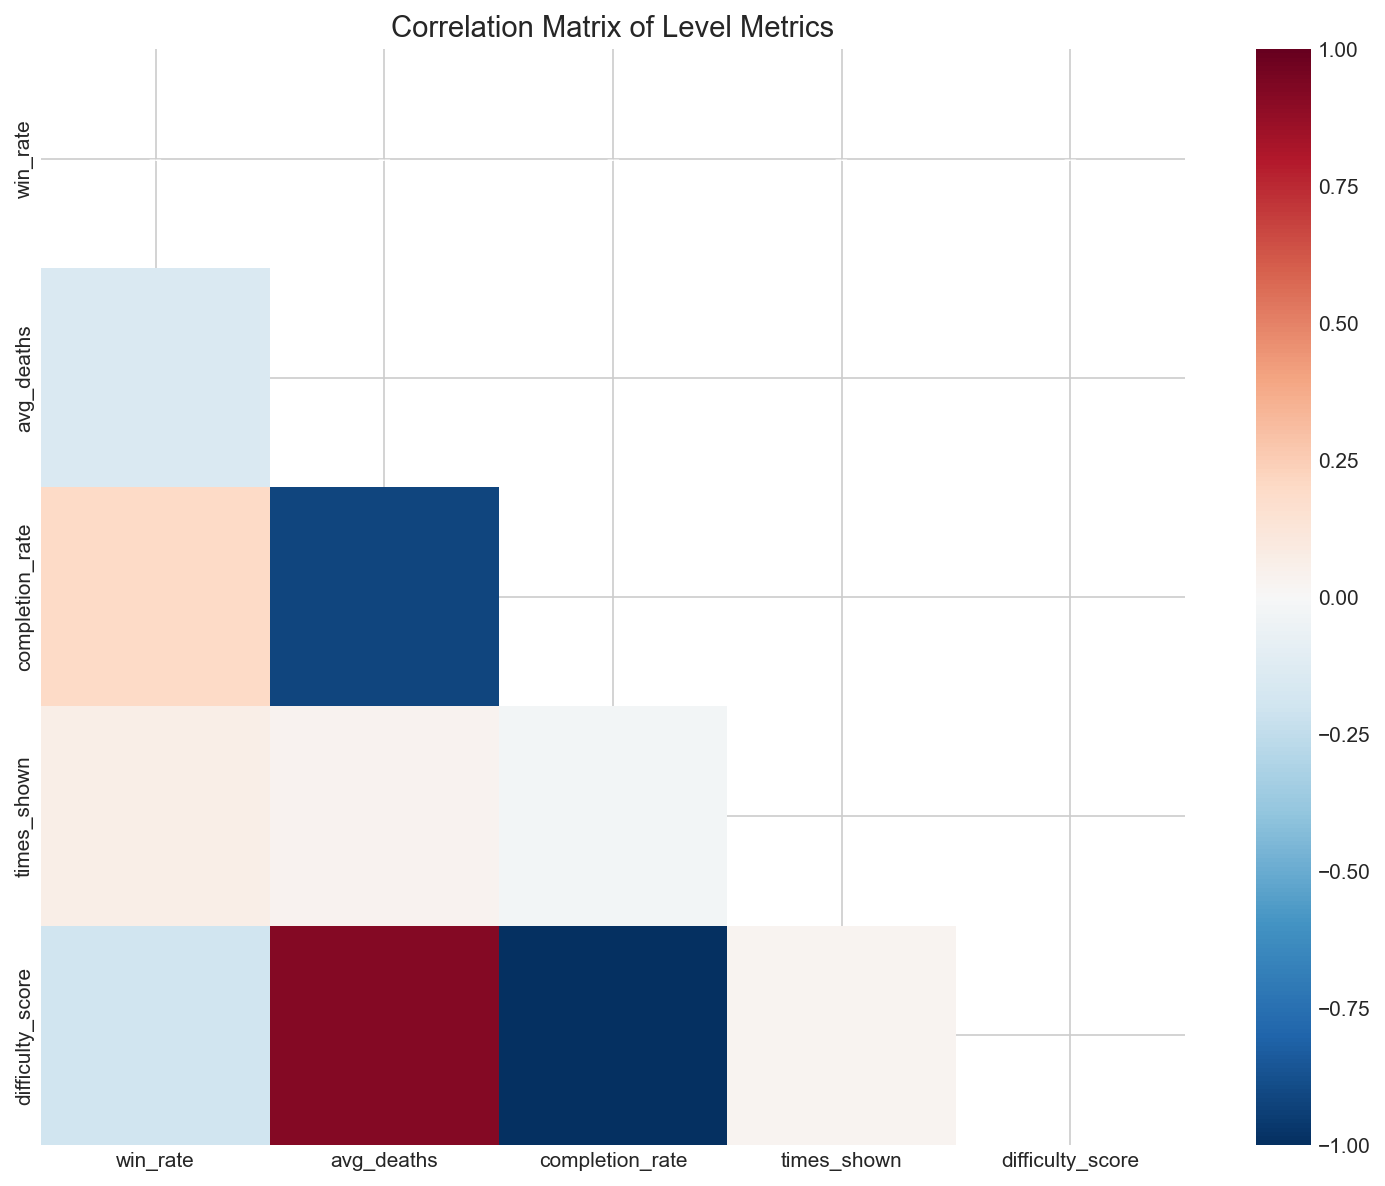
\includegraphics[width=0.85\textwidth]{correlation_matrix.png}
\end{center}
\end{frame}

\begin{frame}
\frametitle{Backup: Feature Importance}
\begin{center}
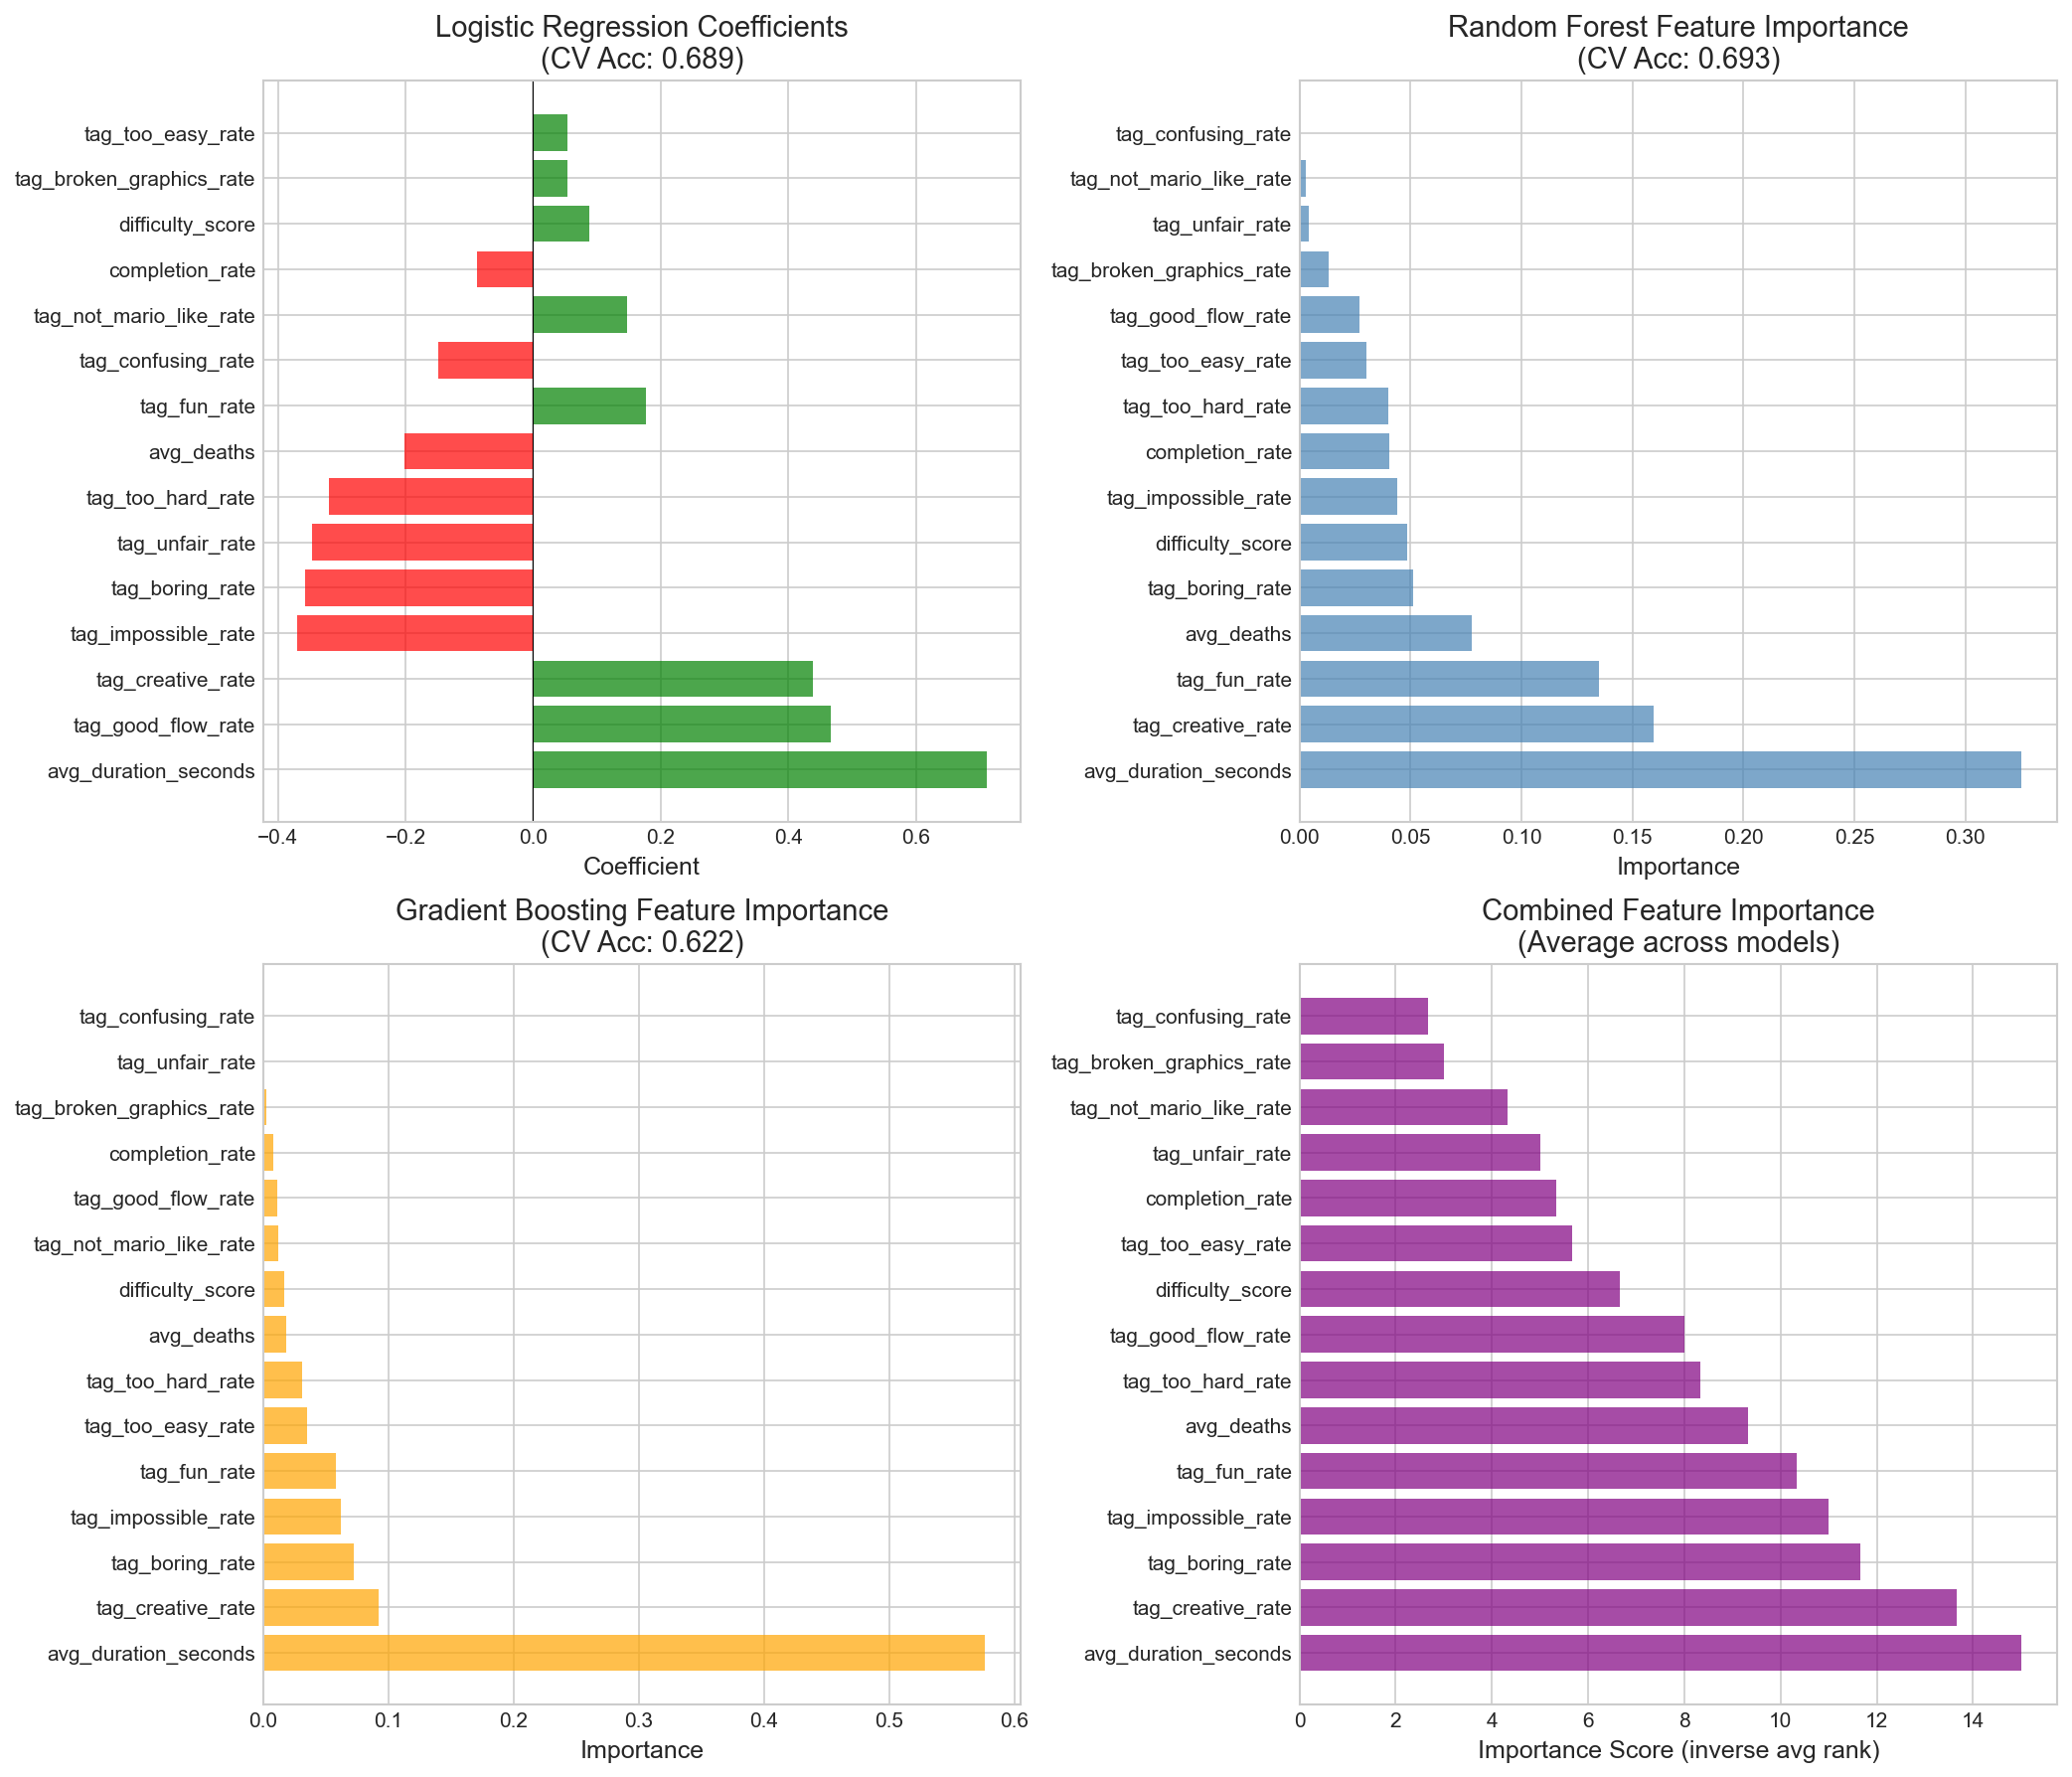
\includegraphics[width=0.85\textwidth]{h10_feature_importance.png}
\end{center}
\end{frame}

\end{document}
